\documentclass[11pt,a4paper]{article}

\usepackage{fontspec}
\setmainfont{Segoe UI}
\setmonofont{Consolas}[Scale=0.88]
\usepackage[margin=25mm]{geometry}
\usepackage{amsmath,amssymb,amsfonts}
\usepackage{graphicx}
\usepackage{booktabs}
\usepackage{tabularx}
\usepackage{array}
\usepackage{listings}
\usepackage{xcolor}
\usepackage{hyperref}
\usepackage{enumitem}
\usepackage{caption}
\usepackage{float}

% --- Hyperlink Setup ---
\hypersetup{
    colorlinks=true,
    linkcolor=blue!70!black,
    citecolor=blue!70!black,
    urlcolor=blue!70!black,
    pdftitle={Adaptive Multi-Market Reinforcement Learning Trading System},
    pdfauthor={BSc Computer Science Candidate}
}

% --- Custom Colors ---
\definecolor{codegreen}{rgb}{0,0.6,0}
\definecolor{codegray}{rgb}{0.5,0.5,0.5}
\definecolor{codepurple}{rgb}{0.58,0,0.82}
\definecolor{backcolour}{rgb}{0.96,0.97,0.98}

% --- Code Listing Setup (Guarantees no operator stripping) ---
\lstdefinestyle{mystyle}{
    backgroundcolor=\color{backcolour},   
    commentstyle=\color{codegreen},
    keywordstyle=\color{blue!80!black}\bfseries,
    numberstyle=\tiny\color{codegray},
    stringstyle=\color{codepurple},
    basicstyle=\ttfamily\footnotesize,
    breakatwhitespace=false,         
    breaklines=true,                 
    captionpos=b,                    
    keepspaces=true,                 
    numbers=left,                    
    numbersep=5pt,                  
    showspaces=false,                
    showstringspaces=false,
    showtabs=false,                  
    tabsize=4,
    frame=single,
    rulecolor=\color{black!15}
}
\lstset{style=mystyle}

% --- Callout Box for Design Connections (Native LaTeX) ---
\newenvironment{callout}{%
  \par\vspace{8pt}
  \noindent\makebox[\linewidth]{\rule{\linewidth}{0.6pt}}\vspace{-4pt}
  \begin{quote}\small
}{%
  \end{quote}\vspace{-6pt}
  \noindent\makebox[\linewidth]{\rule{\linewidth}{0.6pt}}\vspace{8pt}
}

\setlength{\parindent}{0pt}
\setlength{\parskip}{6pt plus 1pt minus 1pt}

\pagestyle{headings}

\begin{document}

% =========================================================================
% FORMAL TITLE PAGE (Native LaTeX)
% =========================================================================
\begin{titlepage}
    \centering
    \vspace*{1.5cm}
    
    {\Huge\bfseries Adaptive Multi-Market\\[0.4em] Reinforcement Learning Trading System \par}
    \vspace{1.0cm}
    
    {\large A Quantitative Trading and Explainable AI Financial Advisory Platform\par}
    
    \vspace{2.5cm}
    
    \rule{0.7\textwidth}{1.2pt}\\[1.5cm]
    
    {\Large\bfseries Final Project Report}\\[1.0cm]
    
    \begin{tabular}{rl}
        \textbf{Module:} & CM3070 Final Project \\
        \textbf{Degree:} & BSc (Hons) Computer Science \\
        \textbf{Institution:} & University of London \\
        \textbf{Date:} & September 2026
    \end{tabular}\par
    \vspace{0.6cm}
    {\small\textbf{Public code repository:} \url{https://github.com/ponggosnayr/cm3070-rl-trading-system}\par}
    
    \vfill
    
    {\small Department of Computing $\cdot$ University of London \par}
\end{titlepage}

% =========================================================================
% ABSTRACT & FRONT MATTER
% =========================================================================
\pagenumbering{roman}

\section*{Abstract}
\addcontentsline{toc}{section}{Abstract}

This project develops an adaptive reinforcement learning trading system and financial advisory dashboard compliant with Project Template Reference 4.2 (Financial Advisor Bot). The objective is to examine whether an autonomous agent can manage trading risk across changing market regimes while providing transparent explanations that retail investors can inspect and understand. To ensure operational clarity and governance, the architecture separates developer-oriented training and validation pipelines from a non-technical web dashboard.

The trading engine pairs Proximal Policy Optimization (PPO) with a 4-layer temporal Transformer feature extractor within a custom Gymnasium environment (\texttt{ActiveCryptoEnv}). The simulation incorporates realistic market execution frictions: next-candle execution ($\text{Open}_{T+1}$), 0.1\% transaction commissions, 0.05\% slippage penalties, trade cooldown constraints, and a clipped log-wealth utility regularized by continuous drawdown and safeguard terms. For decision transparency, the system integrates an Explainable AI (XAI) engine using SHAP (SHapley Additive exPlanations) alongside an action-consistency validator that checks natural-language summaries against underlying neural feature attributions.

The system was evaluated using 5-fold Walk-Forward Validation across 57,756 hourly Bitcoin candles (2020--2026), alongside developer-validation comparisons against DQN, A2C, and passive Buy-and-Hold baselines. Across the five out-of-sample folds, the policy achieved an average Sharpe ratio of 0.60 and a mean out-of-sample ROI of +11.11\% (median +4.73\%), driven by capital preservation during market downturns. In the developer-validation bear-market window, where Buy-and-Hold dropped -24.94\% (52.86\% maximum drawdown), the PPO Transformer policy preserved capital by remaining in cash (0.00\% drawdown), avoiding the losses of the active DQN baseline (-8.04\% ROI, 13.92\% maximum drawdown). In walk-forward bear folds, the policy generated +44.51\% ROI in Fold 2 (market -20.65\%) and +4.73\% ROI in Fold 5 (market -40.89\%). However, strong bull markets resulted in 0 executed trades (Folds 3 and 4), illustrating how fixed downside risk penalties trade off upward momentum capture for downside protection. The project demonstrates the feasibility of risk-averse reinforcement learning for capital preservation while highlighting critical trade-offs in reward formulation, empirical cost thresholds, and explainability validation.

\newpage

% =========================================================================
% TABLE OF CONTENTS & LISTS
% =========================================================================
{
  \hypersetup{linkcolor=black}
  \tableofcontents
  \vspace{1.5cm}
  \listoffigures
  \vspace{1.5cm}
  \listoftables
}

\newpage
\pagenumbering{arabic}

% =========================================================================
% CHAPTER 1
% =========================================================================

\section{Introduction (649/1000 words)}

\subsection{Project Concept and Motivation}
Fixed indicator rules can degrade when market volatility and trends change. Reinforcement Learning (RL) instead learns sequential actions from simulated experience, but financial data are noisy and non-stationary. A policy trained on Bitcoin may fail on other assets, while a complex neural policy may be difficult for retail users to interpret.

I developed an \textbf{Adaptive Multi-Market Reinforcement Learning Trading System} to study these problems. A risk-aware PPO agent with temporal Transformer features chooses among Cash, Long and Short positions. A dashboard presents its signals, historical results and SHAP feature attributions, with rule-based checks on generated explanations. The research tests capital preservation and cross-market transfer while making the system's limitations visible.

The intended users are retail learners who need to inspect a model's evidence before interpreting a signal. A strategy that stays in Cash during a crash may look successful while missing subsequent rallies; backtests therefore compare the agent with both Cash and Buy-and-Hold. Similarly, an explanation that repeats prominent feature names does not by itself show that those features caused a profitable decision. The project evaluates trading behavior, explanation presentation and usability separately so that a strong result in one area cannot hide weakness in another.

\subsection{Project Template Reference}
This CM3070 project follows \textbf{Project Template Reference 4.2 --- Financial Advisor Bot} from the CM3020 Artificial Intelligence track. It separates developer training and validation tools from a React and FastAPI advisory dashboard. Developers can retrain and test policies; users can inspect signals, explanations, backtests and simulations without changing training parameters.

The dashboard runs a saved checkpoint against historical and, when available, current market feeds. Offline labels distinguish historical replay from live quotes. It is a research demonstration and does not place trades on a brokerage account.

\subsection{Research Questions}
The project investigates two questions:
\begin{enumerate}[leftmargin=2em]
    \item \textbf{RQ1:} Can a Transformer-based RL policy preserve capital and limit drawdown against DQN, A2C and Buy-and-Hold across cryptocurrency and transfer markets without excessive trading?
    \item \textbf{RQ2:} Can SHAP attributions and a bounded action-consistency validator produce explanations that rank leading features consistently ($\rho \ge 0.90$) and intercept covered directional contradictions?
\end{enumerate}

\subsection{Project Objectives}
Five objectives guided implementation:
\begin{itemize}[leftmargin=2em]
    \item Ingest historical cryptocurrency, ETF and commodity OHLCV data and compute momentum and volatility features.
    \item Build \texttt{ActiveCryptoEnv} with next-candle execution, fees, slippage and trade cooldowns.
    \item Train a PPO policy with a four-layer Transformer over eight stacked observations.
    \item Evaluate a clipped log-return reward with drawdown and safeguard penalties, including failure modes.
    \item Provide a React/FastAPI dashboard with backtests, SHAP, market regimes and a chatbot with limited consistency checks.
\end{itemize}

\subsection{Ethical Considerations and Regulatory Framework}
This is an experimental decision-support system, not licensed investment advice. The interface labels backtests and chatbot responses as research outputs and does not guarantee capital protection. Cash, Long and Short simulations include cooldown controls, but simulated safeguards cannot remove market risk.

SHAP feature rankings help users inspect signals, while deterministic rules catch only defined directional contradictions in generated text \cite{lundberg2017,arrieta2020}. The system therefore still requires human judgement. API credentials remain in local environment variables, outside the browser; no persistent personal data are required. These choices respond to explainability and privacy concerns in automated decision systems \cite{gdpr2016}.

Historical performance may reflect market-specific conditions, model selection and a limited number of training seeds. The interface should therefore make data freshness, simulated status and downside exposure clear instead of presenting backtest returns as expected future gains.

\newpage

\subsection{Project Planning and Progress Review}
The saved plan scheduled data and web architecture for May--June, model integration for June--July, evaluation for July--August, and final reporting and submission for September. Evaluation continued into report writing because Cash-only policies and incomplete explanation coverage required further diagnostics. Multi-seed performance, complete action coverage and independent user testing remain future work. In retrospect, the plan needed a larger validation buffer and earlier retention of dataset, checkpoint and runtime manifests. The roadmap, calendar and dated September diagnostic records document this change (\path{docs/PROJECT_PLAN.md}; \path{docs/PROJECT_CALENDAR.md}).

\newpage

\section{Literature Review (1724/2500 words)}

\subsection{Reinforcement Learning in Quantitative Finance}
The application of Reinforcement Learning (RL) to automated trading has advanced rapidly over the past two decades. Foundational research by Moody and Saffell (2001) introduced \textbf{Direct Reinforcement Learning (DRL)}, demonstrating that optimizing neural network policies directly on risk-adjusted performance metrics---such as the Differential Sharpe Ratio---yielded more stable trading policies than traditional supervised price forecasting models \cite{moody2001}. Supervised machine learning algorithms attempt to solve price forecasting by predicting future asset prices or directional binary returns ($\text{Sign}(\Delta P_{t+1})$). However, financial time series exhibit low signal-to-noise ratios and heavy-tailed distribution shifts \cite{dixon2020}, causing supervised models to overfit transient noise. Direct RL bypasses price forecasting, optimizing a policy function $\pi_\theta(a_t | s_t)$ that maps market state observations $s_t$ directly to trade actions $a_t$ to maximize cumulative expected return.

With the growth of deep learning, foundational deep Q-learning architectures demonstrated human-level control across complex environments \cite{mnih2015}. In quantitative finance, open-source frameworks such as FinRL \cite{liu2021} and Stable-Baselines3 \cite{raffin2021} popularized deep actor-critic architectures for algorithmic trading and portfolio management. FinRL established a modular three-layer framework (market environment, DRL agent, and application layer) supporting algorithms including Proximal Policy Optimization (PPO), Advantage Actor-Critic (A2C), Deep Deterministic Policy Gradient (DDPG), and Soft Actor-Critic (SAC) \cite{haarnoja2018}. While off-policy algorithms like SAC and Twin Delayed DDPG (TD3) \cite{fujimoto2018} excel in continuous control benchmarks, they require artificial continuous-to-discrete action wrappers for execution spaces with discrete leverage tiers. Consequently, PPO \cite{schulman2017} has become widely adopted in quantitative finance research due to its clipped surrogate objective function, which bounds policy updates during gradient ascent to prevent destructively large policy shifts:
\begin{equation}
L^{\text{CLIP}}(\theta) = \hat{\mathbb{E}}_t \left[ \min\left(r_t(\theta)\hat{A}_t, \, \text{clip}(r_t(\theta), 1-\epsilon, 1+\epsilon)\hat{A}_t\right) \right]
\end{equation}
where $r_t(\theta) = \frac{\pi_\theta(a_t | s_t)}{\pi_{\theta_{\text{old}}}(a_t | s_t)}$ represents the probability ratio between updated and un-updated policies, $\hat{A}_t$ is the Generalized Advantage Estimator (GAE), and $\epsilon$ (typically 0.2) bounds the update step.

Despite the popularity of deep RL trading agents in published literature, recent comprehensive surveys by Pippas et al. (2025) highlight critical methodological vulnerabilities in common RL benchmarks \cite{pippas2025}:
\begin{enumerate}[leftmargin=2em]
    \item \textbf{Oversimplified Market Frictions:} A substantial portion of published literature evaluates RL algorithms in idealized zero-friction environments. In live trading, retail transaction commissions (0.1\%) and market impact slippage (0.05\%) quickly erode high-frequency returns \cite{almgren2000,cartea2015}. Following the transaction cost modeling principles of Almgren and Chriss (2000) and Cartea et al. (2015), the simulation incorporates baseline friction parameters: a 0.1\% commission and 0.05\% slippage allowance per trade. Without explicit fee modeling, RL policies over-trade, generating negative net returns.
    \item \textbf{Look-Ahead Bias in Execution:} Standard RL trading benchmarks evaluate an action selected at step $t$ against the closing price $\text{Close}_t$ of the current candle. Because $\text{Close}_t$ is not finalized until period $t$ concludes, executing orders at $\text{Close}_t$ introduces look-ahead bias. To eliminate look-ahead bias, environments should enforce causal execution conventions, such as next-candle execution against the subsequent opening price $\text{Open}_{T+1}$.
    \item \textbf{State Observation Memory Limits:} Standard Multi-Layer Perceptron (MLP) policy networks process individual state vectors as isolated points in time. This ignores sequential price structures, volatility clustering, and multi-period momentum regimes essential for accurate market evaluation.
\end{enumerate}

\begin{callout}
\textbf{Design Connection:} Following these literature findings, I built \texttt{ActiveCryptoEnv} with explicit $\text{Open}_{T+1}$ execution lag, 0.1\% commission, and 0.05\% slippage. I selected discrete PPO because it natively accommodates the discrete 3-target action space $\{Cash, Long, Short\}$ without the discretization layers required by off-policy continuous algorithms.
\end{callout}

\subsection{Sequence Modeling \& Transformers in Time-Series Finance}
To address the temporal memory limitations of standard MLPs, researchers introduced Recurrent Neural Networks (RNNs) and Long Short-Term Memory (LSTM) networks into RL policy feature extraction layers. LSTMs maintain an internal hidden state cell $h_t$ that carries historical information across consecutive steps. However, LSTMs suffer from gradient vanishing over extended temporal sequences and cannot execute parallel matrix computations across sequence steps during training.

Vaswani et al. (2017) introduced the \textbf{Transformer architecture}, replacing recurrence with multi-head self-attention mechanisms \cite{vaswani2017}. The fundamental scaled dot-product self-attention operation is defined as:
\begin{equation}
\text{Attention}(Q, K, V) = \text{softmax}\left(\frac{QK^T}{\sqrt{d_k}}\right)V
\end{equation}
where $Q$ (Query), $K$ (Key), and $V$ (Value) represent linear projections of the input sequence tensor, and $d_k$ represents the projection feature dimension. Multi-head self-attention extends this mechanism by running $h$ parallel attention heads, enabling the model to jointly attend to information from different representation subspaces at different positions.

Applying Transformer encoders to financial time-series data presents structural challenges. Unlike natural language text, which possesses rigid syntax and semantic tokens, financial price series are non-stationary and noisy. Direct application of standard Transformer encoders without sequence aggregation can lead to overfitting. Lim et al. (2021) demonstrated that incorporating temporal self-attention over multi-horizon time series enables deep models to capture dynamic temporal relationships and regime shifts without recurrence \cite{lim2021}, while Yang et al. (2020) highlighted the efficacy of multi-algorithm deep RL ensembles across fluctuating market conditions \cite{yang2020}.

\begin{callout}
\textbf{Design Connection:} To capture temporal dependencies without overfitting raw price noise, I implemented a 4-layer Deep Transformer Feature Extractor operating over an 8-step frame-stacked observation tensor (136 dimensions), combined with a recency-weighted sequence pooling mechanism (30\% mean pool + 70\% final step) to prioritize recent price action.
\end{callout}

\subsection{Explainable AI (XAI) in Financial Machine Learning}
The transition from interpretable linear models to deep neural sequence architectures created an interpretability barrier in quantitative finance. In financial applications, explainability is a fundamental operational necessity and regulatory requirement \cite{arrieta2020}. Retail users often exhibit reluctance to rely on automated trade recommendations generated by opaque neural networks unless accompanied by inspectable feature attributions \cite{arrieta2020}.

Local feature attribution methods such as LIME \cite{ribeiro2016} and SHAP (SHapley Additive exPlanations) \cite{lundberg2017,lundberg2020} formalize local model interpretability. Grounded in cooperative game theory, SHAP computes Shapley values ($\phi_i$), which measure the fair marginal contribution of feature $i$ across all possible feature sub-combinations $S \subseteq N \setminus \{i\}$:
\begin{equation}
\phi_i(v) = \sum_{S \subseteq N \setminus \{i\}} \frac{|S|!(|N| - |S| - 1)!}{|N|!} \left[ v(S \cup \{i\}) - v(S) \right]
\end{equation}
SHAP provides useful attribution properties for interpreting model outputs:
\begin{itemize}[leftmargin=2em]
    \item \textbf{Local Accuracy (Additive Attribution):} The sum of feature attributions equals the difference between the model prediction for a specific state $f(x)$ and the expected base value: $f(x) = \phi_0 + \sum_{i=1}^M \phi_i$.
    \item \textbf{Consistency:} If a model changes such that the marginal contribution of feature $i$ increases or remains constant, its Shapley value $\phi_i$ will not decrease.
\end{itemize}

While SHAP provides an axiomatic foundation for additive feature attribution, model-agnostic estimators like KernelExplainer approximate Shapley values via weighted local linear regression \cite{lundberg2017}. Recent work by Zeng (2024) explores utilizing Large Language Models (LLMs) to convert numerical SHAP values into natural-language trade narratives \cite{zeng2024}. However, unconstrained LLMs are susceptible to \textbf{hallucination}---generating plausible narratives that contradict mathematical attributions, such as describing a feature as supporting the selected action when its attribution opposes that action.

\begin{callout}
\textbf{Design Connection:} To prevent directional contradictions between language summaries and feature weights, I incorporated an \textbf{action-consistency validator} within the explainability engine. This module audits generated text against SHAP attributions using deterministic lexical rules before presenting explanations to the user (evaluated in Section~\ref{sec:xai_eval}).
\end{callout}

\subsection{Methodological Rigor \& Backtest Overfitting}
A common vulnerability in financial machine learning research is backtest overfitting. Bailey et al. (2017) defined the \textbf{Probability of Backtest Overfitting (PBO)}, proving mathematically that when a strategy configuration is optimized over a single historical path across a large hyperparameter search space, traditional backtest metrics (such as in-sample Sharpe ratio) become statistically unreliable \cite{bailey2014,harvey2015}. High in-sample performance is frequently an artifact of fitting historical noise rather than discovering genuine market alpha.

To enforce quantitative rigor and prevent backtest overfitting, Marcos Lopez de Prado (2018) established core protocol guidelines for financial ML \cite{lopezdeprado2018,bailey2014dsr}:
\begin{enumerate}[leftmargin=2em]
    \item \textbf{Strict Chronological Dataset Splitting:} Shuffle-based cross-validation is methodologically flawed in financial time-series modeling because temporal shuffling destroys autocorrelation and introduces look-ahead data leakage, as technical indicators incorporate overlapping historical window states across adjacent rows.
    \item \textbf{Walk-Forward Validation (WFV):} Strategy evaluation must utilize rolling chronological windows. The policy is trained on fold $k$ and evaluated strictly on out-of-sample fold $k+1$, simulating true chronological deployment.
    \item \textbf{Deflated Sharpe Ratio (DSR):} The Sharpe ratio must be adjusted for non-normality (skewness and kurtosis) of return distributions and corrected for the total number of strategy trials conducted during hyperparameter tuning \cite{bailey2014dsr}.
\end{enumerate}

\begin{callout}
\textbf{Design Connection:} In alignment with chronological evaluation principles, the evaluation framework enforces non-overlapping chronological dataset splits, 5-fold Walk-Forward Validation, and held-out validation checkpointing based on an Objective Score metric.
\end{callout}

\subsection{Application Synthesis \& Identified Research Gap}
To establish a clear justification for this project, existing quantitative trading systems, open-source DRL frameworks, and commercial retail trading platforms were systematically analyzed. 

Early portfolio management frameworks by Jiang et al. (2017) demonstrated that model-free deep RL (using CNNs and LSTMs) could autonomously rebalance cryptocurrency portfolios under simulated fee conditions \cite{jiang2017}. However, their topology relied on static window convolutional filters that cannot capture non-local temporal self-attention across volatile multi-regime time series. Furthermore, open-source development frameworks such as FinRL \cite{liu2021} and standard environments like \texttt{gym-anytrading} focus on developer-facing training pipelines; they lack retail-friendly user interfaces, omit explainability layers, and frequently evaluate policies in simplified zero-slippage or in-sample execution regimes. Conversely, commercial retail bots (such as 3Commas and Kryll.io) provide accessible web dashboards but rely exclusively on rigid, rule-based indicator triggers without adaptive learning or statistical backtest deflations (Table~\ref{tab:framework_comparison}).

\begin{table}[H]
\centering
\footnotesize
\caption{Comparative Matrix: Quantitative Trading Frameworks vs. Proposed System}
\label{tab:framework_comparison}
\begin{tabularx}{\textwidth}{>{\raggedright\arraybackslash}p{2.7cm} >{\raggedright\arraybackslash}X >{\raggedright\arraybackslash}X >{\raggedright\arraybackslash}p{2.4cm} >{\raggedright\arraybackslash}X >{\raggedright\arraybackslash}X}
\toprule
\textbf{Platform / Framework} & \textbf{Execution Friction Realism} & \textbf{Sequence Modeling} & \textbf{Explainability Layer (XAI)} & \textbf{Overfitting Mitigation} & \textbf{Non-Technical Interface} \\
\midrule
\textbf{Standard Baselines (\texttt{gym-anytrading})} & Zero slippage, $\text{Close}_T$ fill & Single-step MLP & Black-box & Single in-sample train/test & CLI script only \\
\addlinespace
\textbf{Jiang et al. (2017) \cite{jiang2017}} & 0.25\% commission & CNN / LSTM & Black-box & In-sample backtest & CLI script only \\
\addlinespace
\textbf{FinRL Framework (Liu et al., 2021) \cite{liu2021}} & Basic commission & Standard MLP / LSTM & Black-box & Basic split cross-validation & Developer Python API \\
\addlinespace
\textbf{Commercial Bots (e.g., 3Commas, Kryll)} & Exchange API execution & None (Heuristic rules) & Fixed rule inspection & Manual parameter tuning & Commercial Web UI \\
\addlinespace
\textbf{Proposed System (This Work)} & \textbf{Next-candle $\text{Open}_{T+1}$, 0.1\% fee, 0.05\% slip} & \textbf{4-Layer Deep Transformer} & \textbf{SHAP + Action-Consistency Validator*} & \textbf{5-Fold WFV + Drawdown-Regularized Utility*} & \textbf{Full-Stack Vite React Web UI} \\
\bottomrule
\end{tabularx}
\caption*{*Note: The environment objective uses clipped log-wealth utility regularized by continuous peak-drawdown and safeguard terms (analyzed in Section~\ref{sec:cash_collapse}). The action-consistency validator is audited using deterministic lexical rules covering target trading terminology.*}
\end{table}

Synthesizing this literature reveals four central research gaps that this project directly addresses:
\begin{enumerate}[leftmargin=2em]
    \item \textbf{The Execution Realism Gap:} Academic RL implementations frequently underperform in live execution due to over-trading driven by zero-friction assumptions and look-ahead bias from executing at current-candle close ($\text{Close}_T$). This project bridges this gap by enforcing next-candle $\text{Open}_{T+1}$ execution lag, 0.30\% round-trip friction (0.15\% per entry/exit), and trade cooldown constraints.
    \item \textbf{The Deep Sequence Representation Gap:} Traditional recurrent networks (LSTMs) suffer from gradient decay across long financial horizons. This work implements multi-head temporal self-attention over an 8-step frame-stacked state representation to dynamically isolate momentum regimes.
    \item \textbf{The Interpretability \& Hallucination Gap:} Deep RL policies remain black boxes to non-technical users, while unconstrained LLM explanations frequently hallucinate polarity reversals. This project integrates local SHAP feature attributions with a limited action-consistency validator to audit natural-language explanations against directional contradictions.
    \item \textbf{The Non-Technical Accessibility Gap:} Existing quantitative DRL platforms are developer-centric tools. This project delivers an intuitive, full-stack web dashboard that decouples model training from non-technical decision inspection, regime monitoring, and risk management.
\end{enumerate}

\section{Design (1381/2000 words)}

\subsection{Dataset Specification \& Split Isolation}
To establish benchmark data, the system ingests historical 1-hour OHLCV candles for Bitcoin (BTC/USDT) sourced from Binance. The available project dataset contains 57,756 hourly rows spanning from 2020-01-04 18:00 to 2026-08-08 13:00. Missing candles are forward-filled to maintain time-series continuity. Because frozen input manifests were not retained across every historical run, these timestamps reflect the preserved dataset prefix. Table~\ref{tab:dataset_splits} outlines the partition boundaries.

\begin{table}[H]
\centering
\footnotesize
\begin{tabularx}{\textwidth}{p{2.8cm} p{3.2cm} c c X}
\toprule
\textbf{Pipeline Workflow} & \textbf{Window Range} & \textbf{Candles} & \textbf{Span} & \textbf{Isolation Guarantee} \\
\midrule
\textbf{Dev Training} & $[0, 46204)$ & 46,204 hrs & Jan 2020 -- Apr 2025 & Single-model training (\texttt{train\_agent.py}) \\
\textbf{Dev Validation} & $[46204, 57756)$ & 11,552 hrs & Apr 2025 -- Aug 2026 & Checkpointing (11,288 test + 264 warm-up) \\
\textbf{Walk-Forward} & $[0, 57756)$ & 57,756 hrs & Jan 2020 -- Aug 2026 & 5 independent expanding folds \\
\bottomrule
\end{tabularx}
\caption{Dataset partition structure and isolation boundaries.}
\label{tab:dataset_splits}
\end{table}

\textbf{Disambiguation \& Out-of-Sample Isolation Guarantee:} It is essential to distinguish between the global 80/20 developer training split (\texttt{train\_agent.py}) and the independent Walk-Forward Validation protocol (\texttt{walk\_forward\_eval.py}):
\begin{enumerate}[leftmargin=2em]
    \item \textbf{Developer Single-Model Training (\texttt{train\_agent.py}):} Uses rows $[0,46204)$ for training and rows $[46204,57756)$ as a held-out validation set. This set selects the persistent dashboard model (\texttt{persistent\_brain.pth}). Of the 11,552 rows in this segment, the initial 264 candles serve as an indicator warm-up window (e.g., to initialize 200-period rolling moving averages and frame buffers), leaving 11,288 stepping candles in the evaluated backtest. In the available data prefix, row 46,204 corresponds to 2025-04-14 06:00.
    \item \textbf{Walk-Forward Validation Protocol (\texttt{walk\_forward\_eval.py}):} Operates completely independently of the global developer validation split to benchmark out-of-sample policy robustness across historical regimes. For each of the 5 WFV folds, a \textbf{fresh, independent PPO Transformer agent} is initialized with random weights and trained strictly on that fold's in-sample expanding window ($0 \dots T_{\text{train}}$) for a fixed budget (30,000 steps) without any checkpoint callbacks or validation early stopping. The trained model is then evaluated once on the subsequent untouched out-of-sample test window ($T_{\text{train}} \dots T_{\text{test}}$). Because each fold trains a fresh throwaway model and uses no validation checkpointing, the test windows of all 5 folds are strictly un-contaminated by model selection leakage.
\end{enumerate}

\subsection{System Architecture \& Decoupled Design}
I designed the system using a decoupled architecture, separating quantitative model training and execution logic from the user-facing web interface. The system comprises five core modules: Multi-Asset Ingestion Pipeline, Gymnasium Environment (\texttt{ActiveCryptoEnv}), Deep Transformer PPO Policy Network, XAI Explainability Engine, and Vite React User Dashboard, as illustrated in Figure~\ref{fig:system_architecture}.

\begin{figure}[h!]
\centering
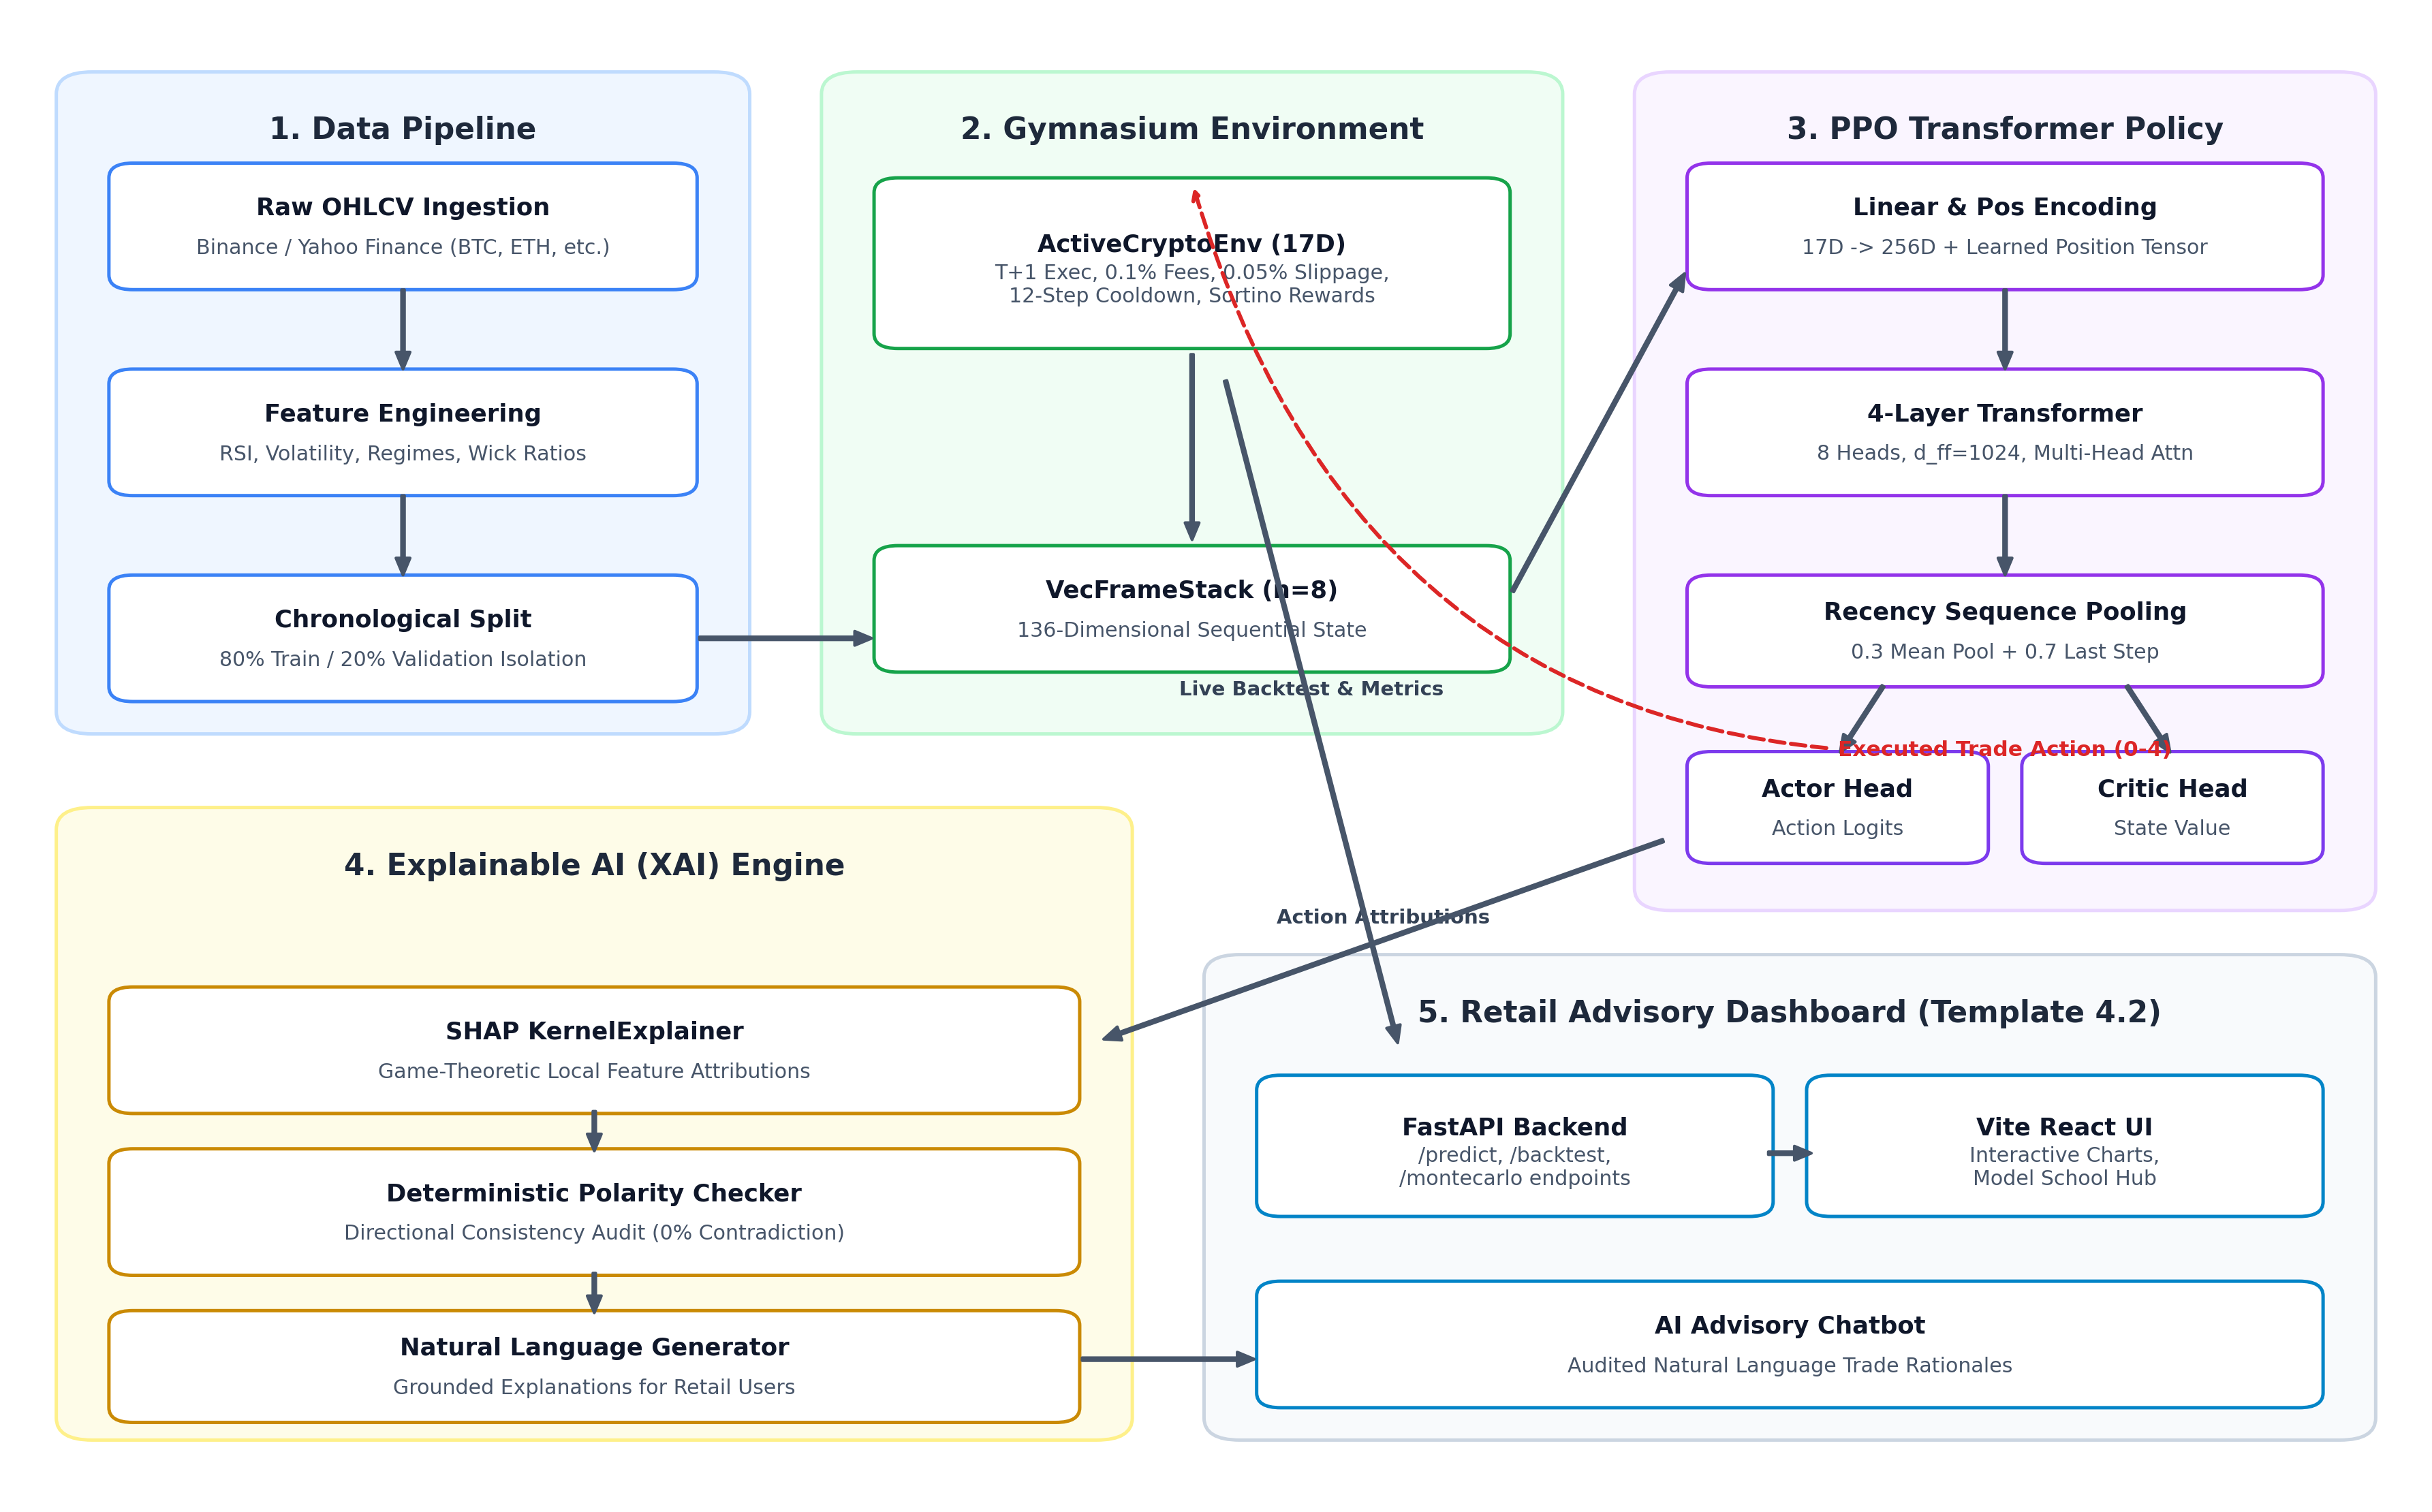
\includegraphics[width=0.92\textwidth]{images/system_architecture.png}
\caption{System architecture and decoupled platform design separating developer training from retail advisory.}
\label{fig:system_architecture}
\end{figure}

\subsection{Gymnasium Environment Design (\texttt{ActiveCryptoEnv})}

\subsubsection{State Space Representation}
I constructed the state observation vector at discrete time step $t$ by combining stationary technical indicators, multi-scale regime context, and portfolio state metrics into a normalized 17-dimensional vector:

\textbf{Group A: Stationary Technical Indicators (7 Dimensions):}
\begin{enumerate}[leftmargin=2em]
    \item \textbf{Candle Body Ratio:} $(Open_t - Close_t) / Close_t \times 200$, clipped to $[-10, 10]$.
    \item \textbf{High-to-Close Spread:} $(High_t - Close_t) / Close_t \times 200$, clipped to $[0, 10]$.
    \item \textbf{Low-to-Close Spread:} $(Low_t - Close_t) / Close_t \times 200$, clipped to $[-10, 0]$.
    \item \textbf{Candle Volatility Ratio:} $(High_t - Low_t) / Close_t \times 200$, clipped to $[0, 10]$.
    \item \textbf{Current Return:} $(Close_t - Close_{t-1}) / Close_{t-1} \times 200$, clipped to $[-10, 10]$.
    \item \textbf{Previous Return:} $(Close_{t-1} - Close_{t-2}) / Close_{t-2} \times 200$, clipped to $[-10, 10]$.
    \item \textbf{Normalized Volume:} $Volume_t / Volume\_SMA_{20} / 5.0$, clipped to $[0, 2]$.
\end{enumerate}

\textbf{Group B: Multi-Scale Context \& Market Regime Features (6 Dimensions):}
\begin{enumerate}[leftmargin=2em, start=8]
    \item \textbf{Short-Term Trend:} $(Close_t - SMA_{20}) / SMA_{20} \times 100$, clipped to $[-5, 5]$.
    \item \textbf{Medium-Term Trend:} $(Close_t - SMA_{99}) / SMA_{99} \times 100$, clipped to $[-5, 5]$.
    \item \textbf{Daily Momentum:} $(Close_t - Close_{t-24}) / Close_{t-24} \times 100$, clipped to $[-5, 5]$.
    \item \textbf{Volatility Ratio:} $Rolling\_Vol_{30} / Vol\_Median_{500}$, clipped to $[0, 3]$.
    \item \textbf{Drawdown from Peak:} $(Close_t - Max\_High_{168}) / Max\_High_{168} \times 100$, clipped to $[-20, 0]$.
    \item \textbf{Market Regime Context:} Discrete regime state ($k \in \{-2, -1, 0, 1, 2\}$) computed causally from an unsupervised 5-state Gaussian Hidden Markov Model fit strictly on in-sample returns, distinguishing Strong Bear, Bear, Sideways, Bull, and Strong Bull regimes.
\end{enumerate}

\textbf{Group C: Portfolio State Features (4 Dimensions):}
\begin{enumerate}[leftmargin=2em, start=14]
    \item \textbf{Position Side:} $1.0$ (Long), $-1.0$ (Short), $0.0$ (Flat).
    \item \textbf{Unrealized PnL:} $(Net\_Worth_t - Balance_{entry}) / Balance_{entry} \times 20$, clipped to $[-1, 1]$.
    \item \textbf{Inactivity Duration:} $\min(1.0, Steps_{flat} / 48.0)$.
    \item \textbf{Position Duration:} $\min(1.0, Steps_{active} / Max\_Duration \times 2.0)$.
\end{enumerate}

To capture temporal sequence dynamics, I wrapped the environment in a \texttt{VecFrameStack} of $n\_stack = 8$, producing a final policy input tensor of dimension $17 \times 8 = 136$ features.

\subsubsection{Action Space \& Execution Frictions}
To eliminate invalid-action masking issues and avoid state-dependent action rejection, the Gymnasium environment (\texttt{ActiveCryptoEnv}) is formulated around a canonical \textbf{3-target-position discrete action space} ($a \in \{0: \text{Cash}, 1: \text{Target Long}, 2: \text{Target Short}\}$):
\begin{itemize}[leftmargin=2em]
    \item \texttt{Action 0: Target CASH (Flat)} --- Maintain flat cash or liquidate an active long/short position.
    \item \texttt{Action 1: Target LONG} --- Open a long position from cash, hold an existing long position (\$0 fee), or flip directly from short to long.
    \item \texttt{Action 2: Target SHORT} --- Open a short position from cash, hold an existing short position (\$0 fee), or flip directly from long to short.
\end{itemize}

This 3-target-position formulation captures the 5 logical trading operations (Hold, Open Long, Close Long, Open Short, Close Short) based on current position state without requiring artificial invalid-action masking wrappers. This representation directly matches the three policy output logits ($[\text{Cash}, \text{Long}, \text{Short}]$) monitored during training and analyzed in the failure diagnostics of Section~\ref{sec:cash_collapse}.

Execution modeling enforces realistic trading frictions:
\begin{enumerate}[leftmargin=2em]
    \item \textbf{Execution Lag:} Actions selected at candle $T$ execute against price $\text{Open}_{T+1}$ of the subsequent candle, eliminating look-ahead bias.
    \item \textbf{Transaction Commission:} $c = 0.1\%$ deducted from trade capital per entry and exit.
    \item \textbf{Slippage Penalty:} $s = 0.05\%$ applied symmetrically against execution price on entry and exit (yielding 0.15\% one-way, 0.30\% round-trip friction).
    \item \textbf{Trade Cooldown Lock:} A cooldown constraint prevents immediate re-entry after liquidation, suppressing high-frequency churn ($\text{trade\_cooldown} = 1$ hour in primary WFV and baseline benchmarks).
\end{enumerate}

\subsubsection{Risk-Adjusted Reward Function Formulation \& Scale Rationale}
To discourage downside capital loss while retaining an activity incentive, the core step-wise reward used by the environment is formulated as:
\begin{equation}
R_t^{\mathrm{core}} = \operatorname{clip}\left(10.0 \cdot \ln\left(\frac{Net\_Worth_t}{Net\_Worth_{t-1}}\right),-1,1\right) - R_{\text{Drawdown}} - R_{\text{Inactivity}}
\end{equation}
\begin{enumerate}[leftmargin=2em]
    \item \textbf{Scaled Log Return ($R_{\text{Return}}$):}
    \begin{equation}
    R_{\text{Return}} = \operatorname{clip}\left(10.0 \cdot \ln\left(\frac{Net\_Worth_t}{Net\_Worth_{t-1}}\right),-1,1\right)
    \end{equation}
    \item \textbf{Peak Drawdown Penalty ($R_{\text{Drawdown}}$):}
    \begin{equation}
    R_{\text{Drawdown}} = 0.1 \times \left( \frac{Peak\_Net\_Worth_t - Net\_Worth_t}{Peak\_Net\_Worth_t} \right)
    \end{equation}
    \item \textbf{Flat Inactivity Decay ($R_{\text{Inactivity}}$):}
    \begin{equation}
    R_{\text{Inactivity}} = I_t
    \end{equation}
    where $I_t$ is a configurable decay penalty applied after an initial flat grace window.
\end{enumerate}

\textbf{Reward Terms and Diagnostic Configuration:} The return multiplier ($10.0\times$) and drawdown coefficient ($0.1\times$) were selected to balance return sensitivity against volatility penalties. The environment implementation also supports optional safeguards and shaping terms: drawdown-cap penalties, duration warnings, conditional profit-realisation bonuses, and post-grace inactivity decay. Activation of these auxiliary terms varies by experimental run. For example, the reward decomposition in Table~\ref{tab:reward_decomposition} reports diagnostic component values where inactivity penalties were disabled and auxiliary shaping terms were recorded separately. An exploratory Sortino-ratio objective was also evaluated during early development, but headline walk-forward results reflect the log-wealth and drawdown specification. A comprehensive sensitivity analysis across individual coefficient weights is left to future work.

\subsection{Deep Transformer Policy Network \& Hyperparameters}
Standard PPO policies utilize Multi-Layer Perceptrons (MLPs) that do not explicitly model temporal dependencies across frame-stacked inputs. I implemented \texttt{DeepTransformerExtractor} to map the 136-dimensional stacked vector back into $(8, 17)$ shape and process it through a temporal encoder (hyperparameters detailed in Table~\ref{tab:hyperparameters}):
\begin{enumerate}[leftmargin=2em]
    \item \textbf{Linear Projection:} Projects each 17D step vector to model dimension $d_{\text{model}} = 256$.
    \item \textbf{Learned Positional Encoding:} Adds a trainable tensor $P \in \mathbb{R}^{1 \times 8 \times 256}$ to preserve step order.
    \item \textbf{Transformer Encoder:} 4 multi-head self-attention layers with $N_{\text{heads}} = 8$ and feedforward expansion $d_{ff} = 1024$.
    \item \textbf{Recency Sequence Pooling:} Standard mean pooling dilutes the importance of the latest price candle. I implemented recency-weighted sequence aggregation:
    \begin{equation}
    Z = 0.3 \times \left( \frac{1}{T} \sum_{i=1}^T H_i \right) + 0.7 \times H_T \quad (T = 8)
    \end{equation}
    where $H_i \in \mathbb{R}^{256}$ is the self-attention output at sequence index $i$.
\end{enumerate}

\begin{table}[H]
\centering
\small
\begin{tabularx}{\textwidth}{l c c X}
\toprule
\textbf{Category} & \textbf{Hyperparameter Symbol} & \textbf{Value} & \textbf{Theoretical Rationale / Usage} \\
\midrule
\textbf{Optimization} & Learning Rate ($\alpha$) & $3 \times 10^{-4}$ (Linear Decay) & Prevents late-stage policy divergence \\
\textbf{Discounting} & Discount Factor ($\gamma$) & $0.97$ ($0.99$ in early exploratory runs) & Primary WFV and training script setting; balances return horizon \\
\textbf{GAE Advantage} & GAE Lambda ($\lambda_{\text{GAE}}$) & $0.92$ ($0.95$ in early exploratory runs) & Primary WFV and training script setting; balances advantage bias vs variance \\
\textbf{PPO Clipping} & Clip Range ($\epsilon$) & $0.20$ & Bounds surrogate policy update steps \\
\textbf{Entropy Scaling} & Entropy Coeff ($c_2$) & $0.01$ ($0.02$ in diagnostics) & Encourages exploration early in training (Table 6 evaluates $0.02$) \\
\textbf{Value Function} & Value Loss Coeff ($c_1$) & $0.50$ & Scales critic loss relative to actor loss \\
\textbf{Batching} & Rollout Steps / Batch Size & 2,048 / 128 & Multi-step vectorized environment sampling \\
\textbf{Epochs} & Epochs per Update ($N_{\text{epochs}}$) & 10 & PPO policy reuse factor per rollout \\
\textbf{Sequence} & Stack ($n_{\text{stack}}$) / $d_{\text{model}}$ & 8 frames / 256 dims & Frame-stacked observation sequence shape \\
\textbf{Attention} & Layers / Heads & 4 layers / 8 heads & Multi-head self-attention depth \\
\textbf{Reproducibility} & Seed Configuration & \texttt{seed = None} (42 in diagnostics) & Production and WFV scripts use framework defaults; diagnostics enforce \texttt{seed = 42} \\
\bottomrule
\end{tabularx}
\caption{Hyperparameter specifications across policy optimization, noting distinctions between primary scripts and exploratory/diagnostic runs.}
\label{tab:hyperparameters}
\end{table}

\textbf{Configuration Reconciliation \& Seed Handling:} The primary codebase implementations in \texttt{src/train\_agent.py} and \texttt{src/walk\_forward\_eval.py} set the discount factor to $\gamma = 0.97$ and GAE parameter to $\lambda_{\text{GAE}} = 0.92$, with framework-managed initialization (\texttt{seed = None}), while controlled ablation scripts enforce \texttt{seed = 42}. Earlier exploratory experiments evaluated $\gamma = 0.99$ and $\lambda = 0.95$. Historical run manifests were not retained for every past experiment, so this report distinguishes between primary codebase settings and controlled diagnostic runs. Furthermore, because each fold used a fixed training budget (30,000 steps) while in-sample training sets expanded from 9,626 hours (Fold 1) to 48,130 hours (Fold 5), later folds completed fewer full passes over their historical data per step budget. Evaluating multi-seed variance and scaling training budgets proportionally with fold length remain areas for future research.

\subsection{Objective Score Checkpointing \& Justification}
To reduce reward-hacking incentives, model checkpoints update only when the \textbf{Objective Score} evaluated every 5,000 steps against a deterministic held-out validation fold improves:
\begin{equation}
\text{Objective Score} = \text{ROI \%} \times \left(1.0 + \max(0.0, \text{Sharpe Ratio})\right)
\end{equation}
\textbf{Justification:} Simple ROI checkpointing rewards high-volatility strategies that achieve transient profits through extreme risk. Conversely, pure Sharpe ratio checkpointing can reward low-return strategies that exhibit minimal variance. Scaling ROI by $(1.0 + \max(0.0, \text{Sharpe}))$ ensures that checkpoint updates prioritize strategies that achieve positive returns paired with consistent risk-adjusted stability.

\section{Implementation (1055/2500 words)}

\subsection{Development Environment \& Codebase Structure}
I developed the system in Python 3.12 utilizing PyTorch \cite{paszke2019}, Gymnasium \cite{towers2024}, and Stable-Baselines3 \cite{raffin2021}, organizing the project into modular packages:

\begin{lstlisting}[language=bash, numbers=none]
FINAL PROJECT/
|-- api.py                    # FastAPI service (Inference, SHAP, Monte Carlo)
|-- train_gui.py              # Tkinter Developer Control Center (CLI/GUI)
|-- src/
|   |-- rl_env.py             # Gymnasium ActiveCryptoEnv & DeepTransformerExtractor
|   |-- train_agent.py        # PPO training loop with dynamic learning rate schedule
|   |-- walk_forward_eval.py  # 5-fold Walk-Forward Validation & risk metrics
|   |-- xai_shap.py           # SHAP KernelExplainer attribution engine
|   |-- xai_engine.py         # Natural Language generator & Action-Consistency Validator
|   |-- xai_audit.py          # Quantitative XAI fidelity evaluation script
|   |-- mc_engine.py          # Monte Carlo equity trajectory simulator
|   `-- trading_utils.py      # Backtest analytics (Sharpe, Sortino, Drawdown)
|-- frontend/                 # Vite React 19 TypeScript Dashboard
|-- tests/                    # Automated Pytest suite (count recorded in project matrix)
`-- models/                   # Saved policy checkpoints (.pth files)
\end{lstlisting}

\newpage

\subsection{Core Algorithmic Code Implementation}

\subsubsection{Environment Step Function and Execution Frictions (\texttt{src/rl\_env.py})}
The environment step function implements next-candle execution timing ($\text{Open}_{T+1}$), proportional transaction fees, slippage, and post-liquidation cooldown locks (abridged implementation excerpt):

\begin{minipage}{\linewidth}
\begin{lstlisting}[language=Python]
def step(self, action: int):
    # Execute at next candle OPEN price to eliminate look-ahead bias
    next_step_idx = min(self.current_step + 1, len(self.df) - 1)
    exec_price = self.df.iloc[next_step_idx]['open']
    
    # 1. Process target position transitions (0: Cash, 1: Long, 2: Short)
    # Frictions: 0.10% commission + 0.05% slippage (0.15% one-way, 0.30% round-trip)
    if action == 0 and (self.is_long or self.is_short):
        self._close_position(exec_price)  # Liquidate to flat cash
    elif action == 1 and not self.is_long:
        if self.is_short:
            self._close_position(exec_price)  # Flip short to long
        self._open_position(side="long", price=exec_price)
    elif action == 2 and not self.is_short:
        if self.is_long:
            self._close_position(exec_price)  # Flip long to short
        self._open_position(side="short", price=exec_price)

    # 2. Advance time step and evaluate mark-to-market net worth at candle close
    self.current_step += 1
    close_price = self.df.iloc[min(self.current_step, len(self.df) - 1)]['close']
    self._update_mark_to_market_net_worth(close_price)

    # 3. Compute step log return and composite risk-adjusted reward
    step_log_return = np.log(self.net_worth / self.prev_net_worth)
    # Penalties include continuous drawdown tax (0.1 * drawdown) and inactivity if active
    reward = np.clip(step_log_return * 10.0, -1.0, 1.0) - self._calculate_penalties()
    self.prev_net_worth = self.net_worth  # Update baseline net worth for next step

    obs = self._get_observation()
    done = self.current_step >= len(self.df) - 1 or self.net_worth <= self.initial_balance * 0.1
    return obs, reward, done, False, {"net_worth": self.net_worth}
\end{lstlisting}
\end{minipage}

\newpage

\subsubsection{Transformer Feature Extractor Architecture (\texttt{src/rl\_env.py})}
The neural policy feature extractor processes stacked sequence frames through 4 multi-head self-attention layers with recency pooling:

\begin{minipage}{\linewidth}
\begin{lstlisting}[language=Python]
class DeepTransformerExtractor(BaseFeaturesExtractor):
    def __init__(self, observation_space: spaces.Box, features_dim: int = 256):
        super().__init__(observation_space, features_dim)
        self.n_stack = 8
        self.n_features = 17
        
        self.input_projection = nn.Linear(self.n_features, 256)
        self.pos_embedding = nn.Parameter(torch.randn(1, self.n_stack, 256))
        
        encoder_layer = nn.TransformerEncoderLayer(
            d_model=256, nhead=8, dim_feedforward=1024, dropout=0.1, batch_first=True
        )
        self.transformer = nn.TransformerEncoder(encoder_layer, num_layers=4)
        self.fc_out = nn.Linear(256, features_dim)

    def forward(self, observations: torch.Tensor) -> torch.Tensor:
        # Reshape (Batch, 136) -> (Batch, 8, 17)
        batch_size = observations.size(0)
        x = observations.view(batch_size, self.n_stack, self.n_features)
        
        # Project and add positional encodings
        x = self.input_projection(x) + self.pos_embedding
        h = self.transformer(x)
        
        # Recency-weighted pooling: 30% mean pool + 70% final step
        mean_pool = h.mean(dim=1)
        last_step = h[:, -1, :]
        pooled = 0.3 * mean_pool + 0.7 * last_step
        return F.relu(self.fc_out(pooled))
\end{lstlisting}
\end{minipage}

\subsubsection{SHAP Attribution and Action-Consistency Validator (\texttt{src/xai\_engine.py})}
The explainability engine calculates SHAP feature attributions conditioned on the policy logit of the selected action $a_t \in \{0, 1, 2\}$. A positive attribution indicates support for that specific action, while a negative attribution indicates opposition. For instance, a positive attribution when Short is chosen reflects evidence favoring short positioning, not general bullishness. The listing below illustrates deterministic formatting of action-conditioned attributions only; it does not implement or certify the narrative validator. A SHAP sign describes a contribution to the selected output relative to its background expectation, not whether the raw feature value is high or low. The separate narrative checks use a bounded lexical rule set; their coverage and limitations are evaluated in Section 5.4:

\begin{minipage}{\linewidth}
\begin{lstlisting}[language=Python]
def format_action_attributions(shap_values, feature_names, action):
    # Illustrative formatter; values explain this selected action's logit.
    indices = np.argsort(np.abs(shap_values))[-3:][::-1]
    statements = []
    for i in indices:
        value = float(shap_values[i])
        if value > 0:
            relation = "supports"
        elif value < 0:
            relation = "opposes"
        else:
            relation = "has zero contribution to"
        statements.append(
            f"{feature_names[i]} {relation} {action} ({value:+.4f})"
        )
    return "; ".join(statements)
\end{lstlisting}
\end{minipage}

\subsubsection{Training Dynamics \& Policy Entropy Monitoring}
\label{sec:training_dynamics}
During PPO optimization, policy loss, value function loss, and policy entropy are tracked across training iterations. In high-friction financial environments, monitoring policy entropy is critical: as analyzed in Section~\ref{sec:cash_collapse}, premature entropy decay toward zero signals policy collapse into deterministic cash holding before the agent can explore viable trade trajectories. Regularizing entropy (\texttt{ent\_coef} = $0.01$) ensures the policy maintains exploration over early training epochs.

\subsection{User-Facing Advisory Dashboard Implementation (\texttt{frontend/src/App.tsx})}
In alignment with Project Template Reference 4.2 guidelines, the user-facing web interface abstracts complex quantitative training logic behind an intuitive, full-stack advisory dashboard built with Vite, React 19, TypeScript, and responsive modular CSS. The application connects asynchronously to the FastAPI backend (\texttt{api.py}), rendering real-time market data, interactive financial charts, and grounded AI explanations:

\begin{enumerate}[leftmargin=2em]
    \item \textbf{Market Overview \& Multi-Asset Selector (Figure~\ref{fig:market_overview}):} Displays monitored cryptocurrency assets and traditional equity ETFs with 24-hour return badges, volatility metrics, live price sparklines, and engine status indicators.
    \item \textbf{Strategy Lab \& Plain-English Rationale (Figure~\ref{fig:simple_mode}):} Features a dual-mode interface designed to minimize cognitive load for non-technical users. The \textbf{Simple Mode} translates multi-factor weights into actionable summaries, policy action probabilities ($P(a_t | s_t)$), defensive capital preservation contexts, and historical case-study evaluations (e.g., 2022 FTX Liquidity Collapse, 2024 ETF Inflow Expansion, High-Volatility Range). An \textbf{Advanced Mode} provides quantitative traders with multi-cycle Sharpe ratios, maximum drawdown metrics, and trade markers.
    \item \textbf{Unsupervised HMM Regime Classifier (Figure~\ref{fig:hmm_regime}):} Visualizes latent market regimes (Bullish Expansion, Sideways Consolidation, Bearish Downturn) identified dynamically by the Gaussian Hidden Markov Model, displaying churn suppression and exposure targets.
\end{enumerate}

\begin{figure}[h!]
\centering
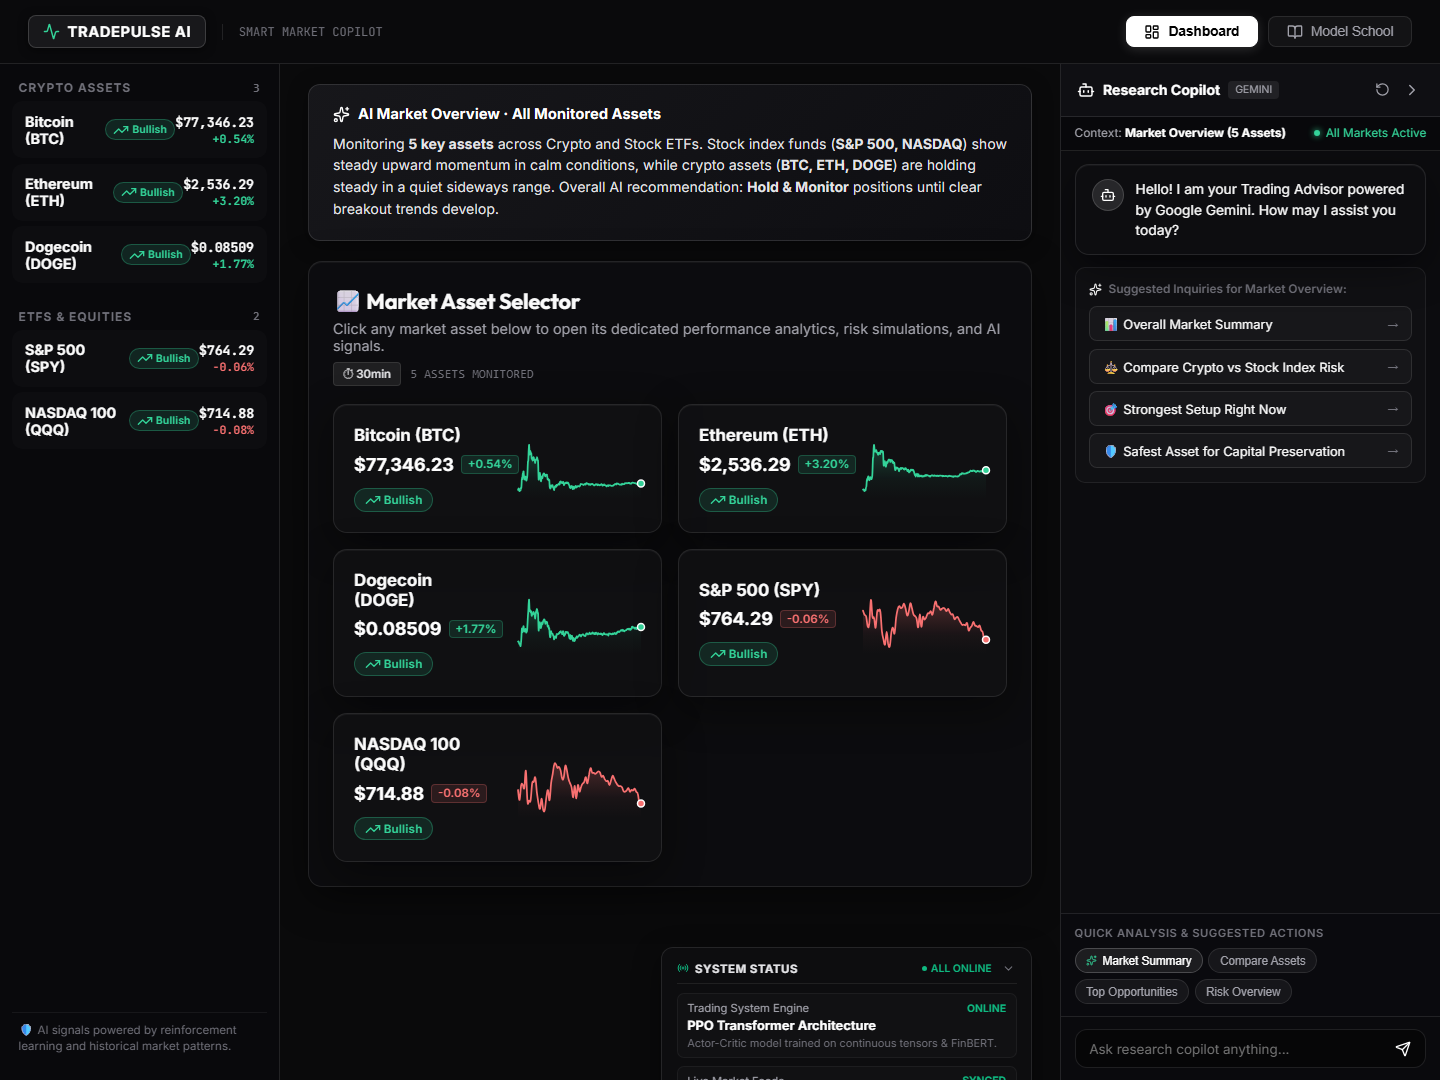
\includegraphics[width=0.82\textwidth]{images/fig_market_overview.png}
\caption{User-facing Multi-Asset Selector and Live Market Overview Dashboard.}
\label{fig:market_overview}
\end{figure}

\begin{figure}[h!]
\centering

\includegraphics[width=0.82\textwidth]{images/fig_simple_mode.png}
\caption{Strategy Lab advisory interface featuring plain-English decision narratives, factor attribution gauges, and historical market case-study evaluations.}
\label{fig:simple_mode}
\end{figure}

\begin{figure}[h!]
\centering
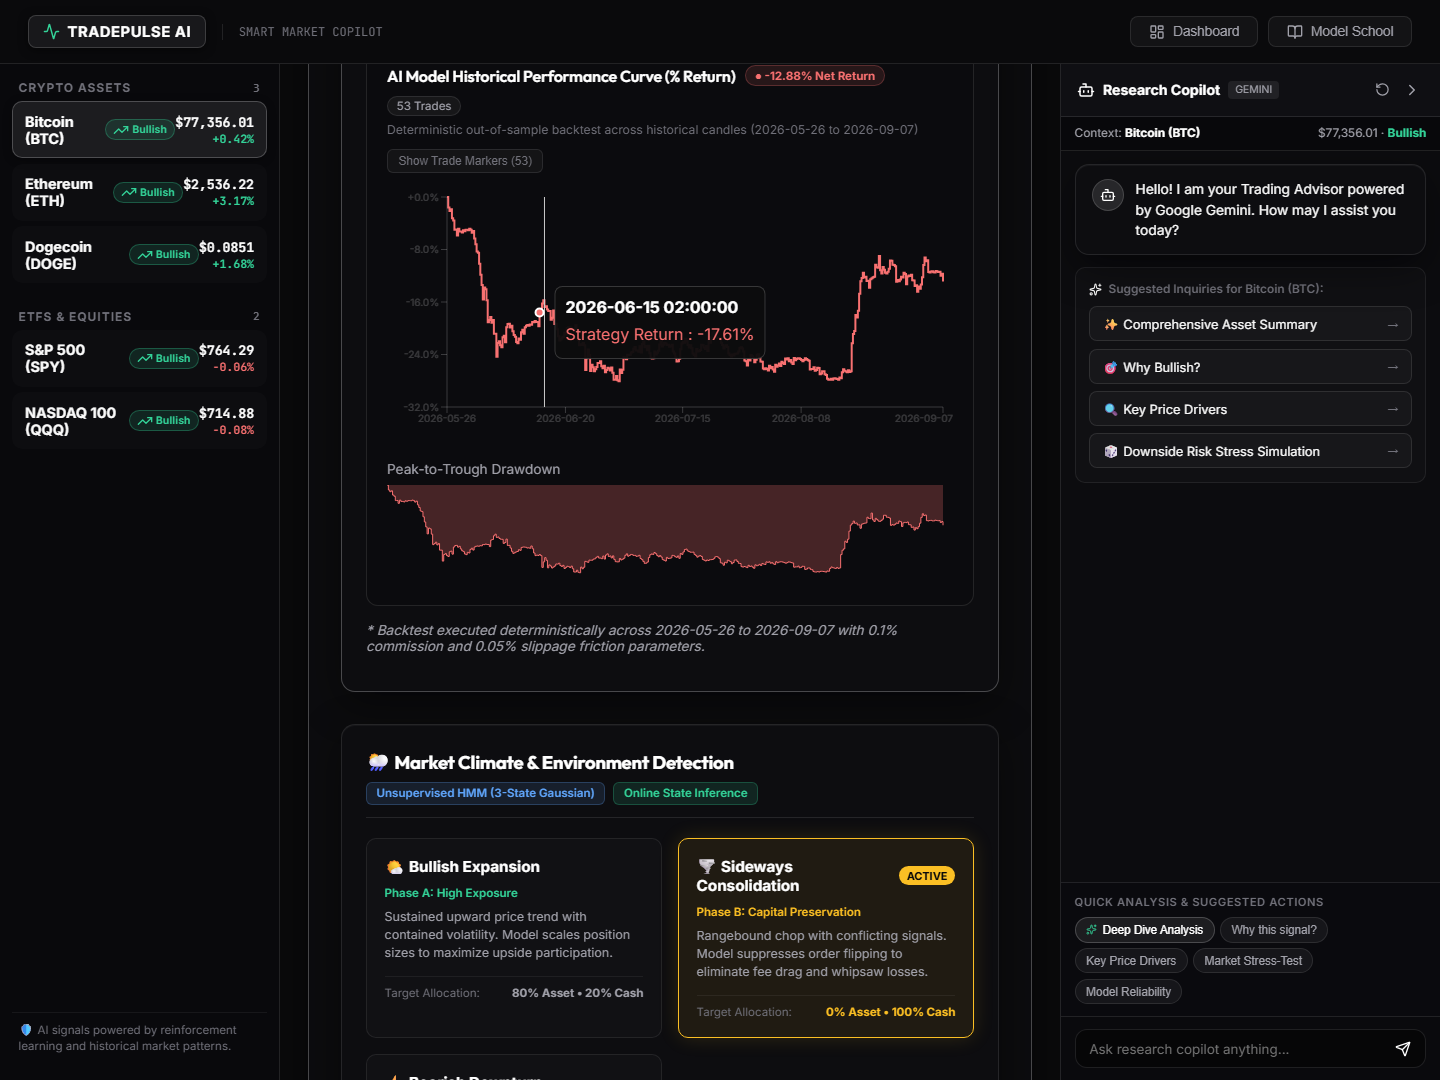
\includegraphics[width=0.82\textwidth]{images/fig_hmm_regime.png}
\caption{Unsupervised Gaussian HMM Market Climate and Regime Inference Interface.}
\label{fig:hmm_regime}
\end{figure}

\newpage

\section{Evaluation (2202/2500 words)}
This chapter separates walk-forward tests, developer validation, diagnostics and historical cross-market results. Their scopes and limits differ.

\subsection{Automated Unit Test Suite \& Latency Benchmarks}
The current suite passed 248 unit and integration tests covering environment transitions, execution frictions, API schemas and XAI rules. This verifies tested behavior, not trading performance or user comprehension. A reproducible decision-step latency benchmark was not retained, so no latency figure is claimed.

\subsection{Walk-Forward and Developer-Validation Results}

\subsubsection{5-Fold Walk-Forward Validation (WFV)}
Five expanding-window folds used 57,756 hourly BTC/USDT candles. Each test interval followed its training interval; Table~\ref{tab:wfv_results} reports out-of-sample results.

\begin{table}[H]
\centering
\footnotesize
\begin{tabularx}{\textwidth}{c c c c c c c c}
\toprule
\textbf{Fold} & \textbf{Train Range} & \textbf{Test Range} & \textbf{ROI} & \textbf{B\&H} & \textbf{Sharpe} & \textbf{Max DD} & \textbf{Trades} \\
\midrule
\textbf{Fold 1} & $[0,9626)$ & $[9626,19252)$ & \textbf{+6.31\%} & +0.52\% & \textbf{0.59} & \textbf{6.74\%} & 2 \\
\textbf{Fold 2} & $[0,19252)$ & $[19252,28878)$ & \textbf{+44.51\%} & -20.65\% & \textbf{1.36} & \textbf{14.35\%} & 65 \\
\textbf{Fold 3} & $[0,28878)$ & $[28878,38504)$ & \textbf{0.00\%} & +123.79\% & \textbf{0.00} & \textbf{0.00\%} & 0 \\
\textbf{Fold 4} & $[0,38504)$ & $[38504,48130)$ & \textbf{0.00\%} & +60.58\% & \textbf{0.00} & \textbf{0.00\%} & 0 \\
\textbf{Fold 5} & $[0,48130)$ & $[48130,57756)$ & \textbf{+4.73\%} & -40.89\% & \textbf{1.04} & \textbf{3.48\%} & 2 \\
\midrule
\textbf{PPO Mean} & --- & --- & \textbf{+11.11\%} & \textbf{+24.67\%} & \textbf{0.60} & \textbf{4.91\%} & \textbf{13.8} \\
\textbf{Cash Benchmark} & --- & --- & \textbf{0.00\%} & \textbf{+24.67\%} & \textbf{0.00} & \textbf{0.00\%} & \textbf{0} \\
\bottomrule
\end{tabularx}
\caption{5-Fold Walk-Forward Validation performance metrics compared against Buy-and-Hold and 100\% Cash reference (Max DD reported as positive percentage loss).}
\label{tab:wfv_results}
\end{table}

\textbf{Statistical Evaluation Scope and Single-Seed Limitation:}
The fold Sharpe mean was 0.60, but no formal empirical Deflated Sharpe Ratio can be inferred without the exploratory trial distribution \cite{bailey2014dsr}. Primary folds used the default framework configuration; controlled diagnostics used \texttt{seed=42}. Without repeated seeds and confidence intervals, initialization variance remains unknown \cite{henderson2018}.

\textbf{Trade Concentration and Inactive Bull Market Positioning (Folds 3 \& 4):}
Of 69 fold trades, 65 occurred in Fold 2, which returned +44.51\% during a -20.65\% market decline. Folds 3 and 4 executed no trades while Buy-and-Hold gained +123.79\% and +60.58\%. Their Cash posture avoided drawdown but missed both rallies.

\textbf{The Risk-Avoidance vs.\ Upside-Participation Trade-off:}
Across folds, PPO's mean ROI was +11.11\% versus Buy-and-Hold's +24.67\%. The Cash-only bull folds suggest that fixed downside penalties and transaction costs can favor exposure avoidance over participation. Reward decomposition below tests this mechanism; the fold results alone do not establish its cause.

\subsubsection{Developer-Validation Baseline Comparison}
Table~\ref{tab:baseline_comparison} compares PPO, DQN, A2C and Buy-and-Hold over 11,288 developer-validation candles after warm-up.

\begin{table}[H]
\centering
\footnotesize
\begin{tabularx}{\textwidth}{p{2.8cm} p{2.6cm} X c c c c}
\toprule
\textbf{Model / Strategy} & \textbf{Architecture} & \textbf{Optimization Objective} & \textbf{ROI (\%)} & \textbf{Max DD (\%)} & \textbf{Trades} & \textbf{Sharpe} \\
\midrule
\textbf{PPO Transformer (Ours)} & 4-Layer Transformer & Clipped log-return + DD & \textbf{0.00\%} & \textbf{0.00\%} & \textbf{0} & \textbf{0.00} \\
\textbf{DQN (Baseline)} & 3-Layer MLP & Action Q-Value Maximization & -8.04\% & 13.92\% & 34 & -0.58 \\
\textbf{A2C (Baseline)} & 3-Layer MLP & Advantage Actor-Critic & 0.00\% & 0.00\% & 0 & 0.00 \\
\textbf{Buy \& Hold (Market)} & Passive Holding & Benchmark Asset Exposure & -24.94\% & 52.86\% & 1 & -0.29 \\
\bottomrule
\end{tabularx}
\caption{Comparative performance evaluation across complete model configurations and market benchmark during the developer-validation period (11,288 evaluated candles; used for checkpoint selection).}
\label{tab:baseline_comparison}
\end{table}

\textbf{Validation scope:} This window informed dashboard checkpoint selection. It is not an independent final test; walk-forward folds used separately trained policies.

PPO stayed in Cash while Bitcoin lost 24.94\%; DQN traded 34 times and lost 8.04\%; A2C also stayed in Cash. The result demonstrates downside avoidance in this selected validation window, without evidence that PPO learned profitable trading there.

\subsection{Failure Analysis: Cash-Collapse Mechanism \& Empirical Ablations}
\label{sec:cash_collapse}
\label{sec:cash_collapse_forensics}
Cash-only convergence in developer validation and six 503,808-step screening runs prompted checks of policy logits, reward components and simplified synthetic trends.

\subsubsection{Measured Policy Saturation and Action Logit Deficit}
I inspected logits from seeds 42, 101 and 777 under harsh and gradual safeguards on bull and bear validation windows:

\begin{table}[H]
\centering
\footnotesize
\begin{tabularx}{\textwidth}{c c c p{2.7cm} p{2.7cm} c c c}
\toprule
\textbf{Seed} & \textbf{Rule} & \textbf{Split} & \textbf{Logits [C, L, S]} & \textbf{Probs [C, L, S]} & \textbf{Max L} & \textbf{Max S} & \textbf{Spread} \\
\midrule
42 & Harsh & Bull & [-0.00, -11.40, -12.45] & [0.99998, 1.1e-5, 4e-6] & 1.1e-5 & 4e-6 & \textbf{+11.40} \\
42 & Gradual & Bull & [-0.00, -11.60, -11.43] & [0.99998, 9e-6, 1.1e-5] & 9e-6 & 1.1e-5 & \textbf{+11.43} \\
101 & Harsh & Bull & [-0.00, -10.38, -10.33] & [0.99994, 3.1e-5, 3.3e-5] & 3.1e-5 & 3.3e-5 & \textbf{+10.33} \\
101 & Gradual & Bull & [-0.00, -10.68, -11.47] & [0.99997, 2.3e-5, 1.0e-5] & 2.3e-5 & 1.0e-5 & \textbf{+10.68} \\
777 & Harsh & Bull & [-0.00, -10.57, -11.52] & [0.99996, 2.6e-5, 1.0e-5] & 2.6e-5 & 1.0e-5 & \textbf{+10.57} \\
777 & Gradual & Bull & [-0.00, -11.89, -12.09] & [0.99999, 7e-6, 6e-6] & 7e-6 & 6e-6 & \textbf{+11.89} \\
\bottomrule
\end{tabularx}
\caption{Measured action logits, action probabilities, and logit spreads across diagnostic 503,808-step PPO screening checkpoints ($\text{ent\_coef}=0.02$).}
\label{tab:checkpoint_logits}
\end{table}

Cash dominated all six checkpoints ($P_{\text{Cash}} \ge 0.99994$); deterministic evaluation selected Cash at every step. Raising diagnostic entropy regularization to 0.02 did not overcome the 10.3--12.5 logit gap.

\subsubsection{Reward-Penalty Decomposition: The Continuous Drawdown Tax}
I logged environment rewards under fixed Cash, Long and Short policies on identical splits, with inactivity penalties disabled (Table~\ref{tab:reward_decomposition}). The columns separate clipped return, per-step drawdown, capital-loss and shaping terms. This diagnostic does not directly measure the critic's value estimates.

\begin{table}[H]
\centering
\footnotesize
\begin{tabularx}{\textwidth}{p{3.2cm} c c c c c c}
\toprule
\textbf{Window / Policy} & \textbf{ROI (\%)} & \textbf{Return Rew.} & \textbf{Step DD Pen.} & \textbf{Cap Pen.} & \textbf{Shaping} & \textbf{Total Rew.} \\
\midrule
\textbf{Bull Val (5,135) -- Cash} & \textbf{0.00\%} & \textbf{0.0000} & \textbf{-0.0000} & \textbf{0.0000} & \textbf{0.0000} & \textbf{0.0000} \\
Bull Val (5,135) -- Long & +32.02\% & +2.7778 & \textbf{-24.5508} & -0.2500 & +3.3139 & \textbf{-18.7092} \\
Bull Val (5,135) -- Short & -29.02\% & -3.4271 & \textbf{-26.5889} & -0.7500 & +3.1616 & \textbf{-27.6044} \\
\midrule
\textbf{Bear Val (5,087) -- Cash} & \textbf{0.00\%} & \textbf{0.0000} & \textbf{-0.0000} & \textbf{0.0000} & \textbf{0.0000} & \textbf{0.0000} \\
Bear Val (5,087) -- Long & -33.36\% & -4.0588 & \textbf{-30.5778} & -0.7500 & +3.7541 & \textbf{-31.6324} \\
Bear Val (5,087) -- Short & +32.53\% & +2.8161 & \textbf{-27.2712} & 0.0000 & +3.8272 & \textbf{-20.6279} \\
\midrule
\textbf{Train Window (45,856) -- Long} & +931.68\% & +24.3800 & \textbf{-204.2037} & -15.0000 & +21.5771 & \textbf{-173.2466} \\
\textbf{2,048-Step Train -- Long} & -15.54\% & -0.4850 & \textbf{-7.8721} & -1.5000 & +2.0747 & \textbf{-7.7824} \\
\textbf{2,048-Step Train -- Cash} & \textbf{0.00\%} & \textbf{0.0000} & \textbf{-0.0000} & \textbf{0.0000} & \textbf{0.0000} & \textbf{0.0000} \\
\bottomrule
\end{tabularx}
\caption{Step-by-step reward and penalty decomposition for fixed policies across validation and training horizons.}
\label{tab:reward_decomposition}
\end{table}

In the bull validation window, fixed Long returned +32.02\% but incurred -24.5508 in accumulated drawdown penalties against +2.7778 in clipped return reward. Its total shaped reward was -18.7092 versus Cash's 0.0000. This supports a reward-design explanation for Cash preference, but does not prove the policy's learned causal mechanism.

\subsubsection{Architectural Verification: Synthetic Trend Benchmark}
In 95-step synthetic tests, a smaller two-layer Transformer returned +27.20\% on a rising series, +17.36\% on a falling series and 0.00\% on a flat series. This checks basic capacity, not real-market performance.

\subsubsection{Empirical Ablations: Drawdown Penalty and Friction Curriculum}
Seed-42 ablations tested the drawdown coefficient and a friction curriculum:

\begin{table}[H]
\centering
\footnotesize
\begin{tabularx}{\textwidth}{p{3.5cm} c p{2.8cm} p{2.8cm} c c}
\toprule
\textbf{Configuration} & \textbf{Budget} & \textbf{Bull Actions [0, 1, 2]} & \textbf{Probs [Cash, Long, Short]} & \textbf{Logit L} & \textbf{Logit S} \\
\midrule
Baseline (\texttt{dd\_coef}=0.1, cd=1) & 32,768 & 5135 / 0 / 0 & [0.8671, 0.0665, 0.0664] & -2.71 & -2.71 \\
Zero DD (\texttt{dd\_coef}=0.0, cd=1) & 32,768 & 5135 / 0 / 0 & [0.8396, 0.0757, 0.0848] & -2.58 & -2.47 \\
Remedy (\texttt{dd\_coef}=0.0, inact, cd=4) & 32,768 & 5135 / 0 / 0 & [0.9098, 0.0460, 0.0443] & -3.08 & -3.12 \\
Direct Full Cost (max\_steps=360) & 49,152 & 5135 / 0 / 0 & [0.9548, 0.0246, 0.0206] & -3.71 & -3.88 \\
\textbf{Curriculum (16k zero $\to$ 32k full)} & 49,152 & 5135 / 0 / 0 & [0.8359, \textbf{0.0898}, \textbf{0.0744}] & \textbf{-2.41} & \textbf{-2.60} \\
\bottomrule
\end{tabularx}
\caption{Empirical ablation results across drawdown coefficient, inactivity incentives, and friction curriculum.}
\label{tab:ablation_results}
\end{table}

Removing the drawdown tax alone left Cash dominant (83.96\%). A 16,384-step zero-friction warm-up raised Long-plus-Short probability to 16.42\%, compared with 4.52\% under direct full-cost training. These short runs improved exploration but still selected Cash on every bull validation step.

\subsubsection{Empirical Analysis: Cost-Induced No-Trade Equilibrium}
The diagnostic mean hourly drift was 0.018\%, versus 0.30\% round-trip friction. Together with drawdown penalties, this makes inactivity attractive under the tested reward. The observed Cash convergence is consistent with a local no-trade equilibrium; testing longer decision intervals remains future work.

\subsection{Explainability \& Action-Consistency Evaluation}
\label{sec:xai_eval}
The multi-action audit in \texttt{src/xai\_audit.py} supplied randomly generated attribution-like arrays to the explanation engine: 50 samples each for Cash, Long and Short. It measured whether generated text preserved the injected top-three feature order, finding mean Spearman $\rho=0.9991$ and no missing features. This is a software check of ordering logic, not evidence that model-derived SHAP explanations are faithful across all three actions (details: \path{docs/XAI_EXPANDED_EVALUATION_2026.md}).

A separate frozen-checkpoint scan found 192 Long actions and no Cash or Short actions in its selected historical slice. It therefore could not test real-model explanation coverage for the other actions. Walk-forward and developer-validation policies had different action patterns and must not be conflated with this checkpoint. Fifty targeted tests check pipeline and polarity rules; the validator catches defined lexical contradictions, not arbitrary semantic errors.

\subsection{Expert Heuristic Usability Evaluation (Nielsen's 10 Heuristics)}
I inspected six dashboard views against Nielsen's usability heuristics \cite{nielsen1994}, focusing on retail comprehension and error recovery.

\subsubsection{Evaluation Scope \& Severity Rating Protocol}
The views covered market signals, backtests, regimes, SHAP, chat and Model School. Defects were graded from 0 (none) to 4 (catastrophic); Table~\ref{tab:heuristic_matrix} records each issue and repair.

\textbf{Methodological Scope and Limitations:}
This was a single internal review, so it cannot establish how independent users would perform. Nielsen's work also shows that multiple evaluators find more defects than one \cite{nielsen1994}.

\subsubsection{Systematic Heuristic Inspection Matrix}
Eight issues and their repairs are listed below.

\begin{table}[H]
\centering
\footnotesize
\renewcommand{\arraystretch}{0.90}
\begin{tabularx}{\textwidth}{c p{2.8cm} p{2.7cm} X c}
\toprule
\textbf{ID} & \textbf{Platform View} & \textbf{Nielsen Heuristic} & \textbf{Audited Usability Defect \& Implemented Solution} & \textbf{Severity} \\
\midrule
\textbf{V-01} & SHAP Importance Tab & H2: Match System \& Real World & \textbf{Defect:} Raw code-level feature names (\texttt{momentum\_rsi\_14}) risked confusing retail users lacking quantitative backgrounds.\newline \textbf{Solution:} Built human-readable aliases and embedded interactive \texttt{InfoBadge} tooltips. & 3 (Major) \\
\midrule
\textbf{V-02} & Backtest / Monte Carlo & H1: Visibility of System Status & \textbf{Defect:} UI froze without feedback during 500-path stochastic calculations, risking perceived platform unresponsiveness.\newline \textbf{Solution:} Implemented animated SVG loading skeletons and progress spinners. & 3 (Major) \\
\midrule
\textbf{V-03} & Advisor Chatbot Tab & H5: Error Prevention / H9: Error Recovery & \textbf{Defect:} Missing or timed-out LLM API keys caused unhandled white-screen promise rejections.\newline \textbf{Solution:} Wrapped execution in try-catch fallback with deterministic template advice. & 3 (Major) \\
\midrule
\textbf{V-04} & Market Overview Tab & H6: Recognition Rather Than Recall & \textbf{Defect:} Lacked interpretive context for non-expert users assessing raw Sharpe ratios or drawdowns.\newline \textbf{Solution:} Added color-coded benchmark badges and direct Model School links. & 2 (Minor) \\
\midrule
\textbf{V-05} & Asset Selector Grid & H4: Consistency \& Standards & \textbf{Defect:} Inconsistent asset naming conventions (\texttt{BTC/USDT} vs.\ \texttt{SPY}).\newline \textbf{Solution:} Standardized asset cards with full names, tickers, and class badges. & 1 (Cosm.) \\
\midrule
\textbf{V-06} & HMM Regime Tab & H8: Aesthetic \& Minimalist Design & \textbf{Defect:} Raw $3 \times 3$ transition probability matrix presented excessive cognitive load for non-technical users.\newline \textbf{Solution:} Replaced matrix with State Pulse Orb and adaptation summary. & 2 (Minor) \\
\midrule
\textbf{V-07} & Backtest Equity Chart & H3: User Control \& Freedom & \textbf{Defect:} Inability to inspect discrete trades on continuous equity curve.\newline \textbf{Solution:} Added interactive Recharts tooltips with buy/sell scatter markers. & 2 (Minor) \\
\midrule
\textbf{V-08} & Model School Hub & H10: Help \& Documentation & \textbf{Defect:} Educational articles were siloed away from active trading analysis views.\newline \textbf{Solution:} Added anchor-linked contextual modal callouts throughout the dashboard. & 2 (Minor) \\
\bottomrule
\end{tabularx}
\caption{Expert Heuristic Usability Evaluation matrix across platform views (Nielsen, 1994 \cite{nielsen1994}).}
\label{tab:heuristic_matrix}
\end{table}

Three issues were rated major, four minor and one cosmetic; all eight received code changes. This is an internal resolution record, not a measured improvement in user outcomes.

\subsection{Interface Usability Evaluation: Cognitive Walkthrough \& Proposed Empirical Protocol}
\label{sec:user_study}
\textbf{Study Scope and Academic Integrity:}
No independent participant study was conducted. An author-led walkthrough with AI assistance used five retail personas to inspect three tasks across the dashboard \cite{wharton1994,nielsen1994}.

\textbf{Standardized Tasks Evaluated:}
\begin{enumerate}[leftmargin=2em]
    \item Interpret the advisor's Cash, Long or Short recommendation.
    \item Identify the leading SHAP feature and direction.
    \item Distinguish live data from offline historical replay.
\end{enumerate}

\textbf{Cognitive Walkthrough Findings and Interface Repairs:}
The walkthrough found three barriers and prompted these interface repairs:
\begin{itemize}[leftmargin=2em]
    \item Raw feature codes obscured SHAP direction; plain-English aliases, a summary banner and tooltips were added.
    \item \texttt{NEUTRAL} was ambiguous; the interface now says \texttt{Target Cash} or \texttt{Stay in Cash}.
    \item Offline status was subtle; an amber badge and historical-replay labels were added.
\end{itemize}

A second author-led pass checked the revised task paths. Independent outcomes remain unknown. A future participant protocol and System Usability Scale instrument are specified in \path{docs/USER_EVALUATION_STUDY.md} \cite{brooke1996,sauro2016}.

\subsection{Zero-Shot Cross-Market Generalization}
I applied a BTC-trained checkpoint to other assets without fine-tuning. Table~\ref{tab:cross_market} preserves the historical results; exact test dates and source-symbol manifests were not retained.

\begin{table}[H]
\centering
\footnotesize
\setlength{\tabcolsep}{3.8pt}
\begin{tabularx}{\textwidth}{l c c c c c c c}
\toprule
\textbf{Target Asset / Class} & \textbf{Candles} & \textbf{Model ROI} & \textbf{B\&H ROI} & \textbf{Excess vs.\ B\&H} & \textbf{Sharpe} & \textbf{Max DD} & \textbf{Trades} \\
\midrule
\textbf{Bitcoin (BTC)} [In-Domain] & 5,000 & \textbf{+8.71\%} & -29.81\% & \textbf{+38.52\%} & \textbf{0.55} & \textbf{33.85\%} & 164 \\
\textbf{Ethereum (ETH)} & 5,000 & \textbf{+14.41\%} & -46.58\% & \textbf{+60.99\%} & \textbf{0.70} & \textbf{30.51\%} & 165 \\
\textbf{Dogecoin (DOGE)} & 5,000 & \textbf{+72.73\%} & -40.60\% & \textbf{+113.33\%} & \textbf{1.79} & \textbf{27.11\%} & 158 \\
\textbf{S\&P 500 ETF (SPY)} & 4,968 & \textbf{-35.08\%} & +67.70\% & -102.78\% & \textbf{-2.25} & \textbf{42.67\%} & 170 \\
\textbf{Nasdaq 100 ETF (QQQ)} & 4,971 & \textbf{-50.46\%} & +93.57\% & -144.03\% & \textbf{-2.92} & \textbf{57.33\%} & 170 \\
\textbf{Crude Oil (WTI)} & 5,000 & \textbf{-51.14\%} & +58.95\% & -110.09\% & \textbf{-1.13} & \textbf{64.78\%} & 162 \\
\textbf{Gold (GLD)} & 5,000 & \textbf{-26.22\%} & +38.11\% & -64.33\% & \textbf{-1.53} & \textbf{38.37\%} & 171 \\
\textbf{Natural Gas (NG)} & 5,000 & \textbf{-7.41\%} & -15.92\% & \textbf{+8.51\%} & \textbf{0.43} & \textbf{53.52\%} & 161 \\
\bottomrule
\end{tabularx}
\caption{Historical zero-shot cross-market results. Exact dates, frequencies, and source-symbol manifests were not retained; GLD is a gold ETF proxy. Max Drawdown is the positive peak-to-trough loss magnitude.}
\label{tab:cross_market}
\end{table}

\textbf{Checkpoint Context:}
This table uses the active \texttt{cross\_market\_eval\_agent.pth}, not the risk-off dashboard checkpoint in Table~\ref{tab:baseline_comparison}. Its Bitcoin reference returned +8.71\% with 164 trades and 33.85\% maximum drawdown.

\textbf{Analysis:} ETH and DOGE beat Buy-and-Hold in these windows, whereas SPY, QQQ, WTI and GLD lost money. Market-hours and liquidity differences are plausible contributors, but cannot be isolated from the retained evidence. GLD is a gold ETF proxy.

\newpage
\section{Conclusion (812/1000 words)}

\subsection{Project Summary \& Achievements}
This project delivered the \textbf{Template 4.2 Financial Advisor Bot} as a trading research system with:
\begin{enumerate}[leftmargin=2em, itemsep=1pt, parsep=0pt]
    \item A Gymnasium simulator with next-candle execution, 0.1\% fees, 0.05\% slippage and downside-risk rewards.
    \item A PPO policy with a four-layer Transformer over eight stacked observations.
    \item Walk-forward evidence of crash-period capital preservation, alongside Cash-only bull folds and weak traditional-market transfer.
    \item SHAP-based dashboard explanations and bounded consistency rules. Synthetic score-array tests checked feature ordering ($\rho=0.9991$); a 192-state real-model scan covered only Long actions.
    \item A React/FastAPI dashboard, eight documented usability repairs and 248 passing automated tests.
\end{enumerate}

\subsection{Evaluation of Research Questions (RQ1 and RQ2)}
\label{sec:rq_evaluation}
The evidence supports both research questions only in part:

\begin{enumerate}[leftmargin=2em]
    \item \textbf{RQ1, partially supported.} Fold 2 returned +44.51\% during a -20.65\% market decline, and the selected developer-validation checkpoint avoided a -24.94\% Bitcoin fall by staying in Cash. ETH and DOGE showed positive historical transfer returns. Yet Folds 3 and 4 missed strong rallies, fold mean ROI (+11.11\%) trailed Buy-and-Hold (+24.67\%), and most traditional-market transfers lost money. The single-seed and checkpoint-selection limits preclude a broad superiority claim.

    \item \textbf{RQ2, partially supported.} Synthetic score-array checks showed consistent feature ordering, and lexical rules caught defined contradictions. The real-model historical scan covered Long only; no independent users tested comprehension, and the validator cannot assess arbitrary semantics. Thus neither full action coverage nor general explanation fidelity is established.
\end{enumerate}

\subsection{Discussion \& Key Insights}
Two primary insights emerged from developing and evaluating the system:
\begin{itemize}[leftmargin=2em, itemsep=2pt, parsep=0pt]
    \item \textbf{Risk Penalties and Regime Trade-offs:} The combination of clipped log returns and continuous drawdown penalties provided effective capital preservation in bear markets, but static penalty weights caused over-conservatism during bull markets. Designing penalties that adapt dynamically to market regimes is essential to avoid trading off upside capture for downside safety.
    \item \textbf{Explainability and Verification in Financial AI:} For retail advisory tools, model recommendations should be inspectable and verifiable. Pairing mathematical attributions (SHAP) with deterministic consistency rules helps ground natural-language summaries, though broad coverage across all action types remains an ongoing challenge.
\end{itemize}

\subsection{Reflection}
Developing this project as the final capstone for the BSc Computer Science highlighted the gap between textbook reinforcement learning and applied work with financial data. In introductory coursework, environments are often stationary and reward feedback is clearer. Financial time-series data is non-stationary, noisy, and path-dependent, so standard policy settings require careful adaptation.

The primary technical challenge was reward formulation rather than model architecture. In early experiments, the agent repeatedly collapsed into inaction: under realistic transaction costs (0.30\% round-trip: 0.15\% entry + 0.15\% exit) and configured downside controls, holding 100\% cash yielded a higher cumulative shaped reward than taking market risk due to drawdown penalties and transaction friction, even during profitable market windows. Addressing this required deconstructing the environment's MDP dynamics, enforcing next-candle execution ($\text{Open}_{T+1}$) to eliminate look-ahead bias, and stacking historical observations to provide temporal momentum context. Additionally, connecting quantitative model outputs to a retail user interface required bounded validation: testing whether generated narratives aligned with underlying SHAP feature attributions showed that trustworthy advisory tools require deterministic guardrails rather than unconstrained generative text.

In hindsight, were I to restart this project, I would alter the development approach in two ways. First, I would implement multi-seed training from the start to quantify policy variance across initialization seeds, rather than evaluating single-seed runs due to local compute constraints. Second, I would dynamically couple reward penalties to market regime classifications (using the Gaussian HMM) directly inside the environment step function, rather than applying static penalties that depress participation during bull markets.

Overall, the project connected concepts from across the degree---deep learning, time-series modeling, asynchronous API development, and human-computer interaction. It reinforced that building machine learning systems requires strict methodological discipline: testing out-of-sample walk-forward performance, running ablation experiments, and objectively documenting failure modes rather than adjusting parameters until backtests look deceptively strong.

\subsection{Future Work}
I identified seven concrete areas for future research and engineering:
\begin{enumerate}[leftmargin=2em, itemsep=2pt, parsep=0pt]
    \item \textbf{Regime-Conditional Reward Adaptation:} Use an unsupervised Hidden Markov Model (\texttt{hmmlearn} \cite{hamilton1989,rabiner1989}) to dynamically modulate drawdown, safeguard, and inactivity terms based on detected market regime.
    \item \textbf{Hyperparameter Sensitivity Analysis:} Conduct systematic grid-search experiments across reward and penalty coefficients ($10.0\times$ return scale, $0.1\times$ drawdown coefficient, safeguard bounds) to map parameter sensitivity.
    \item \textbf{Multi-Seed Evaluation:} Assess policy variance across multiple random seeds ($N=10$) to measure initialization sensitivity.
    \item \textbf{Macro and Sentiment Feature Integration:} Incorporate external market sentiment and macro-economic data into the observation vector.
    \item \textbf{Paper Trading Execution:} Interface the FastAPI backend with exchange APIs (such as CCXT) for live paper trading validation.
    \item \textbf{Action-Conditioned Explainability:} Extend the current selected-logit SHAP approach to multiclass marginal-probability explanations that explicitly capture trade-offs among Cash, Long, and Short.
    \item \textbf{Large-Scale Longitudinal Usability Testing:} Extend the formative usability evaluation protocol (Section~\ref{sec:user_study}) into a formal, ethics-cleared summative empirical study with diverse external retail cohorts ($N \ge 30\text{--}40$) and professional quantitative practitioners, assessing real-time trading comprehension and cognitive load over extended market cycles.
\end{enumerate}

\newpage
\begin{thebibliography}{99}
\small
\setlength{\itemsep}{1.5pt plus 0.5pt minus 0.5pt}
\setlength{\parskip}{0pt}
\bibitem{yang2020} Yang, H., Liu, X.-Y., Zhong, S. and Walid, A. (2020). `Deep Reinforcement Learning for Automated Stock Trading: An Ensemble Strategy', \textit{Proceedings of the First ACM International Conference on AI in Finance (ICAIF)}, pp. 1--8. \url{https://doi.org/10.1145/3383455.3422540}

\bibitem{vaswani2017} Vaswani, A., Shazeer, N., Parmar, N., Uszkoreit, J., Jones, L., Gomez, A.N., Kaiser, \L. and Polosukhin, I. (2017). `Attention Is All You Need', \textit{Advances in Neural Information Processing Systems (NeurIPS)}, 30, pp. 5998--6008. \url{https://arxiv.org/abs/1706.03762}

\bibitem{bailey2014} Bailey, D.H., Borwein, J.M., Lopez de Prado, M. and Zhu, Q.J. (2017). `The Probability of Backtest Overfitting', \textit{Journal of Computational Finance}, 20(4), pp. 39--69. \url{https://doi.org/10.21314/JCF.2016.322}

\bibitem{bailey2014dsr} Bailey, D.H. and Lopez de Prado, M. (2014). `The Deflated Sharpe Ratio: Correcting for Selection Bias, Backtest Overfitting, and Non-Normality', \textit{Journal of Portfolio Management}, 40(5), pp. 94--107. \url{https://doi.org/10.3905/jpm.2014.40.5.094}

\bibitem{schulman2017} Schulman, J., Wolski, F., Dhariwal, P., Radford, A. and Klimov, O. (2017). `Proximal Policy Optimization Algorithms', \textit{arXiv preprint arXiv:1707.06347}. \url{https://arxiv.org/abs/1707.06347}

\bibitem{liu2021} Liu, X.-Y., Yang, H., Gao, J. and Wang, C.D. (2021). `FinRL: Deep Reinforcement Learning Framework to Automate Trading in Quantitative Finance', \textit{ACM International Conference on AI in Finance (ICAIF)}, pp. 1--8. \url{https://arxiv.org/abs/2111.09395}

\bibitem{raffin2021} Raffin, A., Hill, A., Gleave, A., Kanervisto, A., Ernestus, M. and Dormann, N. (2021). `Stable-Baselines3: Reliable Reinforcement Learning Implementations', \textit{Journal of Machine Learning Research}, 22(268), pp. 1--8. \url{http://jmlr.org/papers/v22/20-1364.html}

\bibitem{towers2024} Towers, M., Kwiatkowski, A., Terry, J., Balis, J.U., De Cola, G., Deleu, T., Goul\~ao, M., Kallinteris, A., Krimmel, M., KG, A., Perez-Vicente, R., Pierr\'e, A., Schulhoff, S., Tai, J.J., Tan, H. and Younis, O.G. (2024). `Gymnasium: A Standard Interface for Reinforcement Learning Environments', \textit{arXiv preprint arXiv:2407.17032}. \url{https://arxiv.org/abs/2407.17032}

\bibitem{paszke2019} Paszke, A., Gross, S., Massa, F., Lerer, A., Bradbury, J., Chanan, G., Killeen, T., Lin, Z., Gimelshein, N., Antiga, L., Desmaison, A., K\"opf, A., Yang, E., DeVito, Z., Raison, M., Tejani, A., Chilamkurthy, S., Steiner, B., Fang, L., Bai, J. and Chintala, S. (2019). `PyTorch: An Imperative Style, High-Performance Deep Learning Library', \textit{Advances in Neural Information Processing Systems (NeurIPS)}, 32, pp. 8024--8035.

\bibitem{dixon2020} Dixon, M.F., Halperin, I. and Bilokon, P. (2020). \textit{Machine Learning in Finance: From Theory to Practice}. Cham: Springer International Publishing. \url{https://doi.org/10.1007/978-3-030-41068-1}

\bibitem{almgren2000} Almgren, R. and Chriss, N. (2000). `Optimal Execution of Portfolio Transactions', \textit{Journal of Risk}, 3(2), pp. 5--39. \url{https://doi.org/10.21314/JOR.2001.038}

\bibitem{cartea2015} Cartea, \'A., Jaimungal, S. and Penalva, J. (2015). \textit{Algorithmic and High-Frequency Trading}. Cambridge: Cambridge University Press. \url{https://doi.org/10.1017/CBO9781316054918}

\bibitem{harvey2015} Harvey, C.R. and Liu, Y. (2015). `Backtesting', \textit{The Journal of Portfolio Management}, 42(1), pp. 13--28. \url{https://doi.org/10.3905/jpm.2015.42.1.013}

\bibitem{hamilton1989} Hamilton, J.D. (1989). `A New Approach to the Economic Analysis of Nonstationary Time Series and the Business Cycle', \textit{Econometrica}, 57(2), pp. 357--384. \url{https://doi.org/10.2307/1912559}

\bibitem{rabiner1989} Rabiner, L.R. (1989). `A Tutorial on Hidden Markov Models and Selected Applications in Speech Recognition', \textit{Proceedings of the IEEE}, 77(2), pp. 257--286. \url{https://doi.org/10.1109/5.18626}

\bibitem{mnih2015} Mnih, V., Kavukcuoglu, K., Silver, D., Rusu, A.A., Veness, J., Bellemare, M.G., Graves, A., Riedmiller, M., Fidjeland, A.K., Ostrovski, G., Petersen, S., Beattie, C., Sadik, A., Antonoglou, I., King, H., Kumaran, D., Wierstra, D., Legg, S. and Hassabis, D. (2015). `Human-level control through deep reinforcement learning', \textit{Nature}, 518(7540), pp. 529--533. \url{https://doi.org/10.1038/nature14236}

\bibitem{haarnoja2018} Haarnoja, T., Zhou, A., Abbeel, P. and Levine, S. (2018). `Soft Actor-Critic: Off-Policy Maximum Entropy Deep Reinforcement Learning with a Stochastic Actor', \textit{International Conference on Machine Learning (ICML)}, PMLR 80, pp. 1861--1870. \url{https://arxiv.org/abs/1801.01290}

\bibitem{fujimoto2018} Fujimoto, S., Hoof, H. and Meger, D. (2018). `Addressing Function Approximation Error in Actor-Critic Methods', \textit{International Conference on Machine Learning (ICML)}, PMLR 80, pp. 1587--1596. \url{https://arxiv.org/abs/1802.09477}

\bibitem{lundberg2017} Lundberg, S.M. and Lee, S.-I. (2017). `A Unified Approach to Interpreting Model Predictions', \textit{Advances in Neural Information Processing Systems (NeurIPS)}, 30, pp. 4765--4774. \url{https://arxiv.org/abs/1705.07874}

\bibitem{lundberg2020} Lundberg, S.M., Erion, G., Chen, H., DeGrave, A., Prutkin, J.M., Nair, B., Katz, R., Himmelfarb, J., Bansal, N. and Lee, S.-I. (2020). `From local explanations to global understanding with explainable AI for trees', \textit{Nature Machine Intelligence}, 2(1), pp. 56--67. \url{https://doi.org/10.1038/s42256-019-0138-9}

\bibitem{ribeiro2016} Ribeiro, M.T., Singh, S. and Guestrin, C. (2016). `"Why Should I Trust You?": Explaining the Predictions of Any Classifier', \textit{ACM SIGKDD International Conference on Knowledge Discovery and Data Mining (KDD)}, pp. 1135--1144. \url{https://doi.org/10.1145/2939672.2939778}

\bibitem{arrieta2020} Arrieta, A.B., D\'iaz-Rodr\'iguez, N., Del Ser, J., Bennetot, A., Tabik, S., Barbado, A., Garcia, S., Gil-Lopez, S., Molina, D., Benjamins, R., Chatila, R. and Herrera, F. (2020). `Explainable Artificial Intelligence (XAI): Concepts, taxonomies, opportunities and challenges toward responsible AI', \textit{Information Fusion}, 58, pp. 82--115. \url{https://doi.org/10.1016/j.inffus.2019.12.012}

\bibitem{zeng2024} Zeng, X. (2024). `Enhancing the Interpretability of SHAP Values Using Large Language Models', \textit{arXiv preprint arXiv:2409.00079}, version 1. \url{https://arxiv.org/abs/2409.00079v1}

\bibitem{pippas2025} Pippas, N., Ludvig, E.A. and Turkay, C. (2025). `The Evolution of Reinforcement Learning in Quantitative Finance: A Survey', \textit{ACM Computing Surveys}, 57(11), Article 295, pp. 1--51. \url{https://doi.org/10.1145/3733714}

\bibitem{jiang2017} Jiang, Z., Xu, D. and Liang, J. (2017). `A Deep Reinforcement Learning Framework for the Financial Portfolio Management Problem', \textit{arXiv preprint arXiv:1706.10059}. \url{https://arxiv.org/abs/1706.10059}

\bibitem{moody2001} Moody, J. and Saffell, M. (2001). `Learning to Trade via Direct Reinforcement', \textit{IEEE Transactions on Neural Networks}, 12(4), pp. 875--889. \url{https://doi.org/10.1109/72.935097}

\bibitem{lopezdeprado2018} Lopez de Prado, M. (2018). \textit{Advances in Financial Machine Learning}. New York: John Wiley \& Sons.

\bibitem{lim2021} Lim, B., Ar\i k, S.\,O., Loeff, N. and Pfister, T. (2021). `Temporal Fusion Transformers for Interpretable Multi-horizon Time Series Forecasting', \textit{International Journal of Forecasting}, 37(4), pp. 1748--1764. \url{https://doi.org/10.1016/j.ijforecast.2021.03.012}

\bibitem{gdpr2016} European Parliament and Council of the European Union (2016). `Regulation (EU) 2016/679 (General Data Protection Regulation)', \textit{Official Journal of the European Union}, L119, pp. 1--88.

\bibitem{fca2022} Financial Conduct Authority (2022). `Strengthening our financial promotion rules for high-risk investments and firms approving financial promotions', \textit{FCA Policy Statement PS22/10}. London: Financial Conduct Authority. \href{https://www.fca.org.uk/publications/policy-statements/ps22-10-strengthening-our-financial-promotion-rules-high-risk-investments-firms-approving-financial-promotions}{Official FCA page}.

\bibitem{sec2020} Securities and Exchange Commission (2020). `Commission Guidance Regarding the Proxy Voting Responsibilities of Investment Advisers', \textit{SEC Release No. IA-5547}. Washington, D.C.: U.S. Securities and Exchange Commission.

\bibitem{bis2022} Bank for International Settlements (2022). `Prudential Treatment of Cryptoasset Exposures', \textit{Basel Committee on Banking Supervision Standards}. Basel: Bank for International Settlements.

\bibitem{wharton1994} Wharton, C., Rieman, J., Lewis, C. and Polson, P. (1994). `The cognitive walkthrough method: A practitioner's guide', in Nielsen, J. and Mack, R.L. (eds.) \textit{Usability Inspection Methods}. New York: John Wiley \& Sons, pp. 105--140.

\bibitem{nielsen1994} Nielsen, J. (1994). `Heuristic evaluation', in Nielsen, J. and Mack, R.L. (eds.) \textit{Usability Inspection Methods}. New York: John Wiley \& Sons, pp. 25--62.

\bibitem{sauro2016} Sauro, J. and Lewis, J.R. (2016). \textit{Quantifying the User Experience: Practical Statistics for User Research}. 2nd ed. Cambridge, MA: Morgan Kaufmann.

\bibitem{brooke1996} Brooke, J. (1996). `SUS: A `quick and dirty' usability scale', in Jordan, P.W., Thomas, B., Weerdmeester, B.A. and McClelland, I.L. (eds.) \textit{Usability Evaluation in Industry}. London: Taylor \& Francis, pp. 189--194.

\bibitem{henderson2018} Henderson, P., Islam, R., Bachman, P., Pineau, J., Precup, D. and Meger, D. (2018). `Deep Reinforcement Learning that Matters', \textit{Proceedings of the AAAI Conference on Artificial Intelligence}, 32(1), pp. 3207--3214.
\end{thebibliography}

\end{document}

